In this chapter, we examine the effect of including tetraquark operators on the spectrum determination in the scalar meson sectors containing the $K_0^*(700)$ (previously the $K_0^*(800)$, here and often elsewhere referred to as the $\kappa$) and the $a_0(980)$. It has been suggested before that the $\kappa$ and $a_0(980)$ could have tetraquark content~\cite{Jaffe:2004ph, Amsler:2004ps, Close:2002zu, Maiani:2004uc}, and to date, there have been a small number of studies investigating tetraquarks on the lattice using light quarks. In 2010, Prelovsek et al.\ investigated the $\sigma$ and $\kappa$ as possible tetraquark candidates, but neglected disconnected diagrams in their calculations~\cite{Prelovsek:2010kg}. Using tetraquark interpolators, they found an additional light state in both the $\sigma$ and $\kappa$ channels. In 2013, the ETM collaboration examined the $a_0(980)$ and $\kappa$ using four-quark operators~\cite{Alexandrou:2012rm}, though they also neglected disconnected diagrams in their calculations. They found no evidence of an additional state that can be interpreted as a tetraquark. In 2018, Alexandrou et al.\ conducted a study of the $a_0(980)$ with four-quark operators~\cite{Alexandrou:2017itd}, including disconnected contributions. In their study, they found an additional finite-volume state in the sector containing the $a_0(980)$ meson, which has primarily quark-antiquark content but also has sizeable diquark-antidiquark content, in the range of 1100 to 1200 MeV. Additionally, they conclude that disconnected diagrams have drastic effects on their results, and thus cannot be neglected. The importance of including disconnected diagrams when studying the $\kappa$ and $a_0(980)$ (as well as other scalar mesons) is also shown in Ref.~\cite{Guo:2013nja}. We make two different determinations of the spectrum in each symmetry channel: one using a basis of only single- and two-meson operators, and one using a basis that also includes a tetraquark operator selected from hundreds of tetraquark operators which were tested. We find that including a tetraquark operator yields an additional low-lying finite-volume state in each symmetry channel. In this work, we use the stochastic LapH method~\cite{Morningstar:2011ka} to evaluate the diagrams in our calculations, including \textit{all} disconnected contributions.
\section{Ensemble}\label{sec:ensemble}
We perform Monte Carlo calculations using $412$ gauge field configurations generated by the Hadron Spectrum collaboration~\cite{Edwards:2008ja, Lin:2008pr} on an anisotropic lattice of size $32^3\times 256$ with a length of $3.74$ fm and a pion mass of approximately $230$ MeV, using $N_f=2+1$ Wilson clover fermions. Ensemble details are given in Table~\ref{table:ensemble}, and the action is described in Sec.~\ref{sec:improved_action} and Sec.~\ref{sec:tuning}.
\renewcommand{\arraystretch}{1.0}
\begin{table}
  \centering
  \begin{tabular}{|l|l|l|l|l|l|}
    \hline
    $(L/a_s)^3 \times (T/a_t)$ & $N_{\rm{configurations}}$ & $a_t m_\pi$ & $a_t m_K$ & $a_t$ & $\xi$ \\
    \hline
    $32^3\times 256$ & $412$ & $0.03953(17)$ & $0.08348(14)$ & $0.033357(59)$ fm & $3.451(11)$\\
    \hline
  \end{tabular}
  \caption[Details of the ensemble used in this work.]{Details of the ensemble used in this work. The temporal lattice spacing is taken from Ref.~\cite{Brett:2018jqw}. The renormalized anisotropy $\xi$ is taken from Ref.~\cite{Bulava:2016mks}.}\label{table:ensemble}
\end{table}
\renewcommand{\arraystretch}{1.5}
\section{Operator Construction}
We include single- and two- meson operators, as well as tetraquark operators, in the basis of interpolating operators. As a brief review of the material presented in Ch.~\ref{ch:operators}, we construct our elemental operators using building blocks of smeared, gauge-covariantly displaced quark fields, and stout-smeared link variables. To form the final operators out of our elemental operators, we project the elemental operators onto various symmetry channels according to isospin, parity, $G$-parity, octahedral little group, etc. That is, to form a meson operator $M_{l}(t)$ that transforms irreducibly under all symmetries of interest (labeled by the compound index $l$) at time $t$, we must 
take a linear combination of our elemental meson operators, $M_{l}(t)=c_{\alpha \beta}^{(l)} \Phi_{\alpha \beta}^{A B}(\boldsymbol{p}, t)$. To form a two-meson operator $\mathcal{O}_l(t)$, we would follow a similar procedure and project the product of two final meson operators $M^{a}_{l_a}(t) M^{b}_{l_b}(t)$ onto a final symmetry channel $l$: $\mathcal{O}_l(t) = c^{(l)}_{l_a l_b} M^{a}_{l_a}(t) M^{b}_{l_b}(t)$.

Recall that in order to construct a tetraquark operator, we must consider the various ways to construct a color-singlet four-quark object out of four quark fields. As seen in Ref.~\cite{pittir33243}, the Clebsch-Gordon decompositions show that the only way to construct a color-singlet is by using two quarks and two antiquarks, and that doing so yields two linearly independent color singlet objects:
\begin{equation}\label{eq:cg}
\begin{array}{l}
    {3 \otimes 3 \otimes 3 \otimes 3=3\oplus3\oplus3\oplus\overline{6}\oplus\overline{6}\oplus15\oplus15\oplus15\oplus15},\\
    {3 \otimes 3 \otimes 3 \otimes \overline{3}=\overline{3}\oplus\overline{3}\oplus\overline{3}\oplus6\oplus6\oplus6\oplus\overline{15}\oplus\overline{15}\oplus24},\\
    {3 \otimes 3 \otimes \overline{3} \otimes \overline{3}=1\oplus1\oplus8\oplus8\oplus8\oplus8\oplus10\oplus\overline{10}\oplus27}.
\end{array}
\end{equation}
There are 81 basis vectors formed by the quark fields, $p_{a}^{*}(x) q_{b}^{*}(x) r_{c}(x) s_{d}(x)$, where each $r$, $s$ transforms as a color vector in the fundamental $3$ irrep, and so, $p^{*}$, $q^{*}$ transform in the $\overline 3$ irrep. The following combinations are both linearly independent and gauge-invariant,
\begin{equation}\label{eq:tsta}
\begin{aligned} T_{S} &=\left(\delta_{a c} \delta_{b d}+\delta_{a d} \delta_{b c}\right) p_{a}^{*}(x) q_{b}^{*}(x) r_{c}(x) s_{d}(x), \\ T_{A} &=\left(\delta_{\alpha c} \delta_{b d}-\delta_{\alpha d} \delta_{b c}\right) p_{\alpha}^{*}(x) q_{b}^{*}(x) r_{c}(x) s_{d}(x),\end{aligned}
\end{equation}
and so they form a basis with which to construct our elemental tetraquark operators, fulfilling the need for \emph{two} linearly independent color singlet operators from Eq.~(\ref{eq:cg}).

While we chose only a handful of tetraquark operators for our final analysis, we designed hundreds of operators with differing flavor structures, color structures (i.e.\ the symmetric and antisymmetric combinations of Eq.~(\ref{eq:tsta})), and displacements. We tested these operators by individually adding them to a basis of single- and multi-meson operators to see if an additional level was found in an initial low-statistics analysis on 25 gauge configurations. Most of the operators did not yield an additional level, but we found particular operators that did. In the $\kappa$ channel, we tested several flavor structures, the shorthand representative names of which are: $\overline s u \overline s s$, $\overline s u \overline u u$, and $\overline s u \overline d u$. Table~\ref{table:flavor_structs} gives the relation between these representative flavor structures and the actual flavor content they represent. Moving forward, when we refer to flavor structures, we will use their shorthand names. We found that only operators with the $\overline s u \overline s s$ flavor structure yielded an additional finite-volume state, and that the additional state was present with both color structures. In our initial low-statistics analysis, we tested both single-site and quadruple displacements, and found operators of both types that seemed to yield additional finite-volume states; however, the quadruply-displaced operators came at a significantly higher computational cost and introduced either additional noise or no improvement, and so were excluded from the final operator sets. In the $a_0(980)$ channel, we tested several flavor structures, the shorthand representative names of which are: $\overline u u \overline d u$, $\overline s s \overline d u$, and $\overline d u \overline d u$. We found that only operators with the $\overline u u \overline d u$ flavor structure yielded an additional finite-volume state. As in the $\kappa$ channel, we found that both color structures were able to produce an additional level. After finding no improvement with other displacement types in the $\kappa$ channel, we chose to only test single-site operators in the $a_0(980)$ channel. In both channels, we also constructed operator bases that included several tetraquark operators, and found that the number of additional levels in the energy range we examined was unchanged.

\begin{table}
  \centering
  \begin{tabular}{|l|l|l|}
    \hline
    Representative flavor & Flavor content & Isospin\\
    \hline
    $\overline u u \overline d u$ & $(\overline{u} u+\overline{d} d) \overline{d} u$ & 1\\
    $\overline s s \overline d u$ & $\overline s s \overline d u$ & 1\\
    $\overline d u \overline d u$ & $\overline{d} u(\overline{u} u-\overline{d} d)-(\overline{u} u-\overline{d} d) \overline{d} u$ & 1\\
    $\overline s u \overline s s$ & $\overline s u \overline s s$ & $\frac{1}{2}$\\
    $\overline s u \overline u u$ & $\overline{s} u(\overline{u} u+\overline{d} d)$ & $\frac{1}{2}$\\
    $\overline s u \overline d u$ & $\overline{s} u(\overline{u} u-\overline{d} d)-\sqrt{2} \overline{s} d \overline{d} u$ & $\frac{1}{2}$\\
    \hline
  \end{tabular}
  \caption[Flavor content of our tetraquark operators which are chosen to match those of our two-meson operators.]{Flavor content of our tetraquark operators which are chosen to match those of our two-meson operators. The operators in the last column refer to annihilation operators.}\label{table:flavor_structs}
\end{table}

\section{$\kappa$ Channel}
\subsection{Operator Bases}
The quantum numbers associated with the $\kappa$ are $I(J^{P})=\frac{1}{2}(0^+)$ and $S=1$ , which means that on the lattice we work in the isodoublet, strange, $A_{1g}$ symmetry sector (see Table~\ref{table:O_occurrence_nums}). Below a cutoff of approximately 1.5 times the mass of the nucleon, where the $K_0^*(1430)$ resonance is expected, we expect to see only multi-hadron states. Since we are examining the effect of tetraquark operators on just the low-lying states, we therefore primarily include two-hadron operators. It is always a good idea to add one or more single hadron operators, however, as any operator with the correct quantum numbers can excite states in the spectrum. The operator basis we use, not including any tetraquark operators, is shown in Table~\ref{table:kappa_ops_no_tq}.
\begin{table}
  \centering
  \begin{tabular}{l|l}
    \textbf{Single-Hadron Operators} & \textbf{Two-Hadron Operators}\\
    \hline
    $K_{A_{1g}}^{DDL2}$ & $K(0)_{A_{1u}}^{SS0}\pi(0)_{A_{1u}^-}^{SS0}$\\
    $K_{A_{1g}}^{TDO3}$ & $K(0)_{A_{1u}}^{SS0}\eta(0)_{A_{1u}^+}^{SS0}$\\
    $K_{A_{1g}}^{TDU5}$ & $K(0)_{A_{1u}}^{SS0}\phi(0)_{A_{1u}^+}^{SS0}$\\
    & $K(1)_{A_2}^{SS1}\pi(1)_{A_2^-}^{SS1}$\\
    & $K(1)_{A_2}^{SS1}\eta(1)_{A_2^+}^{SS1}$\\
    & $K(1)_{A_2}^{SS1}\phi(1)_{A_2^+}^{SS1}$\\
    & $K(2)_{A_2}^{SS0}\pi(2)_{A_2^-}^{SS0}$\\
    & $K(3)_{A_2}^{SS0}\pi(3)_{A_2^-}^{SS0}$
  \end{tabular}
  \caption[Operators used in the $\kappa$ channel, excluding tetraquark operators.]{Operators used in the $\kappa$ channel, excluding tetraquark operators. Particle names refer to \emph{flavor content} and should not be taken literally. $K$ refers to $u\overline s$, $\pi$ refers to $u\overline d$, $\eta$ refers to $u\overline u + d\overline d$, and $\phi$ refers to $s\overline s$ flavor structure. The number in parentheses following the particle name denotes the square of its total momentum in lattice units, the superscript denotes displacement type, and the subscript denotes octahedral irrep and $G$-parity.}
  \label{table:kappa_ops_no_tq}
\end{table}

Our final class of tetraquark operators used in this channel were single-site $\overline s u \overline s s$, with both the symmetric and antisymmetric color structures included. The final tetraquark operator chosen was a $\overline s u \overline s s$, antisymmetric, single-site operator, which we denote as \verb+tqsuss2m SS2+. Of the tetraquark operators that produced an additional level, we chose this one due to its high signal quality.
\subsection{Spectrum Determination}
For all results in this chapter, we use the kaon mass as a reference. The fit used to determine the kaon mass is shown in Fig.~\ref{fig:kaon}. For all fits in this channel, the normalization time, metric time, and diagonalization time used in the GEVP were $\tau_N=3$, $\tau_0=6$, and $\tau_d=12$, respectively. While we expect that the single-pivot method described in Sec.~\ref{sec:pivots} ensures that the correlator matrix remains diagonal at all times, it is sometimes difficult to ensure that off-diagonal elements of the correlator matrix are statistically consistent with zero at all times. Choosing later diagonalization times helps with this, but comes with the tradeoff of introducing more noise. We found that choosing $\tau_d=12$ yielded a good combination of reduced noise and a near-sufficiently diagonal matrix. Still, there were some off-diagonal elements which were slightly farther than zero than we would hope, so we took care to extract the spectrum at three different diagonalization times and confirm that our energies were consistent across these diagonalization times. Our results are shown in Fig.~\ref{fig:spectrum_td}.

Fits to the diagonalized correlator set for the operator basis containing no tetraquark operators are shown in Fig.~\ref{fig:kappa_no_tq_grid}, and the operator overlap factors are shown in Fig.~\ref{fig:kappa_no_tq_zfactors}. Fit details are given in Table~\ref{table:kappa_no_tq_spectrum}. Recall from Sec.~\ref{sec:correlator_matrices} that we must use more operators in our basis than energies we wish to reliably extract, so there are fewer fits shown than operators used. (This will often be the case throughout this work.) Fits using the same operator basis, but with the addition of the $\overline s u \overline s s$ tetraquark operator, are shown in Fig.~\ref{fig:kappa_with_tq_grid}, and the operator overlap factors are shown in Fig.~\ref{fig:kappa_with_tq_zfactors}. Fit details are given in Tables~\ref{table:kappa_with_tq_spectrum}. We prefer to use two-exponential fits wherever possible, though it is sometimes necessary to use single-exponential fits to achieve precise energy determinations. We choose the beginning of the fit range $t_{\rm{min}}$ by fitting to several values and choosing the earliest value at which the fit value becomes stable, in order to determine when excited state contamination stops altering our result. The end of the fit range $t_{\rm{max}}$ is chosen to be approximately the time at which the principle correlator becomes statistically consistent with zero, since fitting to points with a low signal-to-noise ratio is undesirable.

A plot comparing our determinations of the low-lying spectrum for each basis is shown in Fig~\ref{fig:kappa_spectrum}. The result is clear: including the tetraquark operator yields an additional level at $E/m_K = 2.139(62)$. Without including such a tetraquark operator, we miss an energy level in the spectrum determination. Recall from the spectral decomposition of the correlator matrix in Eq.~(\ref{eq:corr_spec_decomp}) that in order to extract the energy of a state $\ket{n}$, we must have an operator $\overline O$ that creates a state with overlap onto $\ket{n}$, i.e.\ $\bra{n}\overline O\ket{0}$ must be large enough to be measurable. Additionally, we see that the energy determinations for the other levels shift slightly, which is to be expected when one attempts to extract a spectrum with an operator basis that is not sufficiently saturated with operators.~\cite{Dudek:2012xn} Taking a look at the overlap factors, we see that there is significant overlap between this additional level (level 3) and the state created by the tetraquark operator, as well as significant overlap between this additional level and the state created by the $K(0)\phi(0)$ operator. No other operators create states that significantly overlap onto this tetraquark state. We also see that both of these operators overlap onto the state just below it (level 2), which is very near in energy. Therefore, without the tetraquark operator, the $K(0)\phi(0)$ operator on its own is unable to resolve both levels, and produces a level between the two, as we see in the left spectrum determination of Fig.~\ref{fig:kappa_spectrum}. This significant result suggests that there is a state in the finite-volume lattice spectrum that shares quantum numbers with the $\kappa$ resonance, and that has tetraquark content.

% Firm evidence of the $\kappa$ resonance having tetraquark content will have to wait for future scattering studies employing
A more detailed examination of the role of the tetraquark operator for the $\kappa$ resonance will require the L\"uscher method~\cite{Luscher:1990ck} with increased statistics and tetraquark operators of nonzero momenta. The L\"uscher method is a formalism that relates discrete finite-volume spectra to infinite-volume scattering amplitudes. It is worth noting that one such study of the $\kappa$ resonance by Brett et al.~\cite{Brett:2018jqw}, using the same ensemble used here, gave a qualitative determination of the $\kappa$ mass to be $4.66(11)m_\pi$ from an effective range parameterization and $4.59(11)m_\pi$ from  a Breit-Wigner parameterization. Both of these masses are within error of the mass of our additional finite-volume state, which is $4.52(13)m_\pi$ (the pion mass fit used to determine this ratio is shown in Fig.~\ref{fig:pion}). Additionally, the consequences of missing a finite-volume energy such as the one found in this work may be severe for variants of L\"uscher's method that fit scattering parameters by comparing the finite-volume spectrum predicted by a particular scattering amplitude to that obtained on the lattice, such as the method used by the Hadron Spectrum Collaboration in Ref.~\cite{Wilson:2015dqa}. However, for variants of L\"uscher's method that rely on computing scattering parameters from finite-volume energies, such as the determinant residual method~\cite{Morningstar:2017spu} used by Brett et al.\, the consequences should not be as severe.

\begin{figure}
  \centering
  \begin{subfigure}{0.4\textwidth}
    \centering
    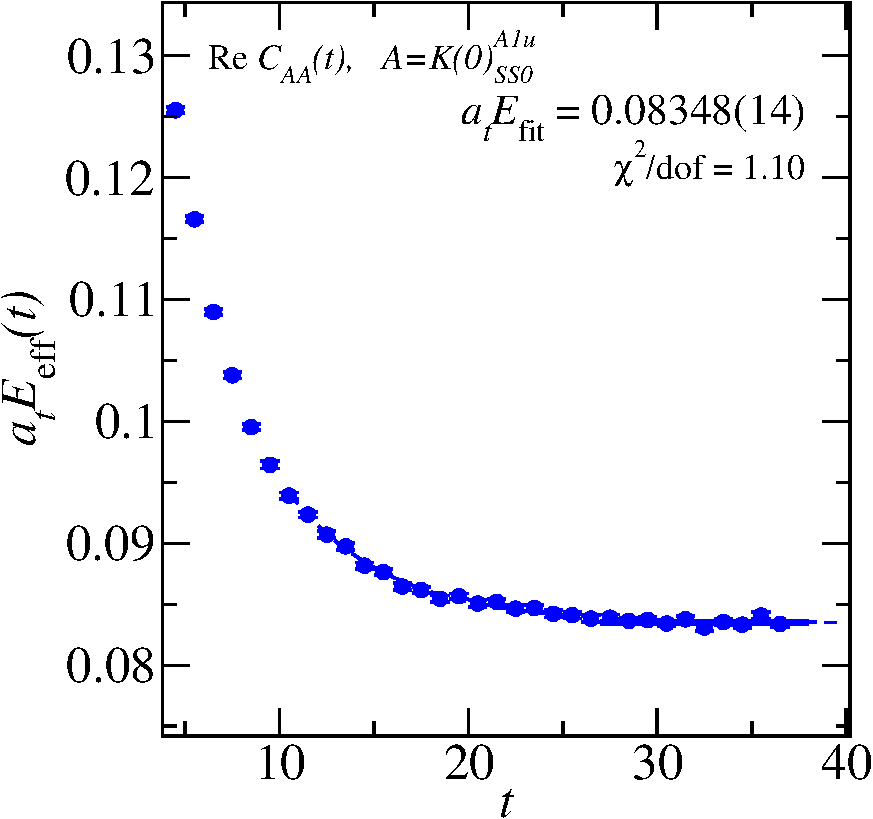
\includegraphics[width=\textwidth]{figures/kaon_crop.pdf}
    \caption{Kaon mass}\label{fig:kaon}
  \end{subfigure}\hfill
  \begin{subfigure}{0.4\textwidth}
    \centering
    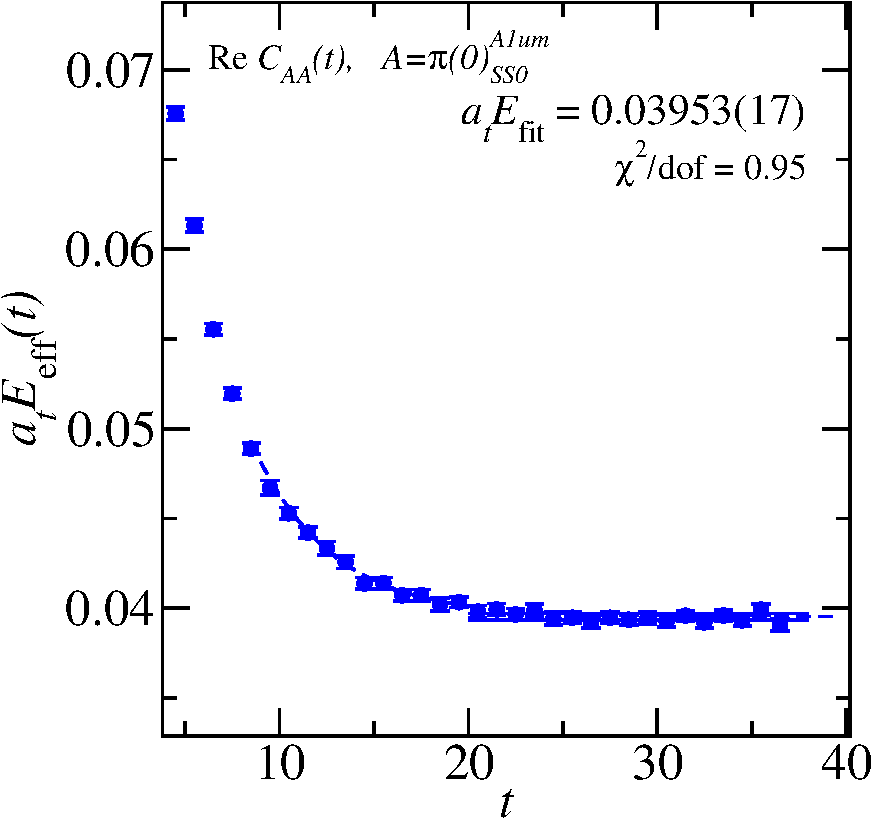
\includegraphics[width=\textwidth]{figures/pion_crop.pdf}
    \caption{Pion mass}\label{fig:pion}
  \end{subfigure}
  \caption{Fits to the reference masses, used in this chapter.}
\end{figure}


\begin{figure}
  \raisebox{-.08cm}{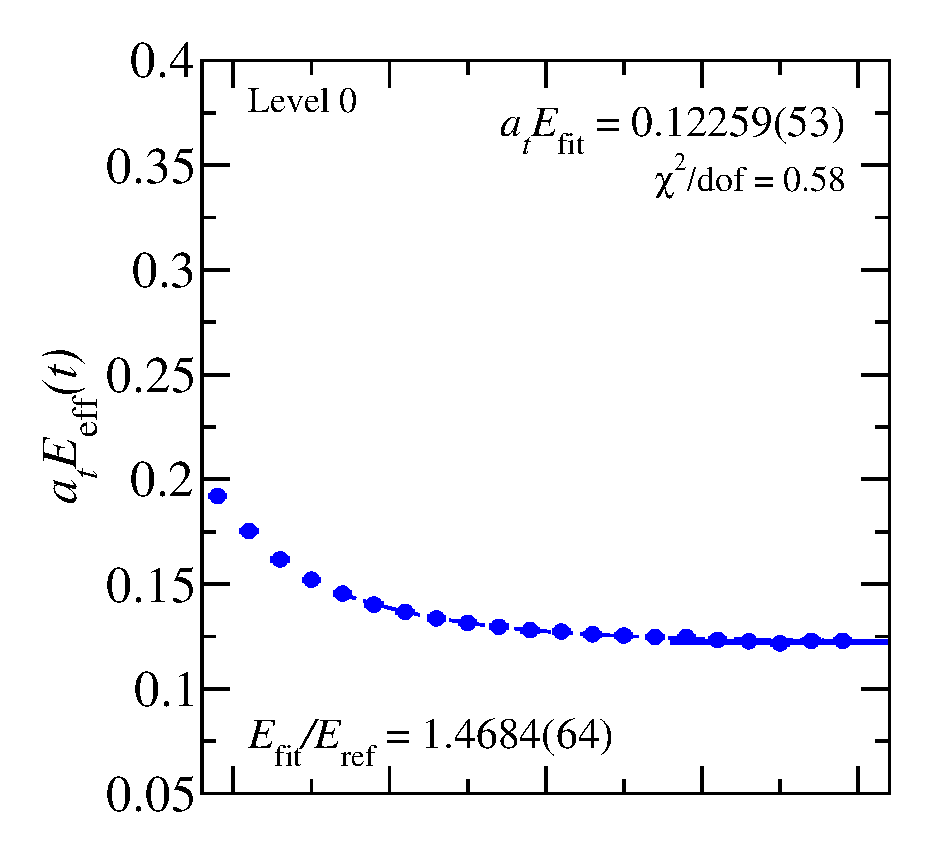
\includegraphics[width=0.336\textwidth]{figures/spectrum_a1g/no_tq/fits/fit_0.pdf}}
  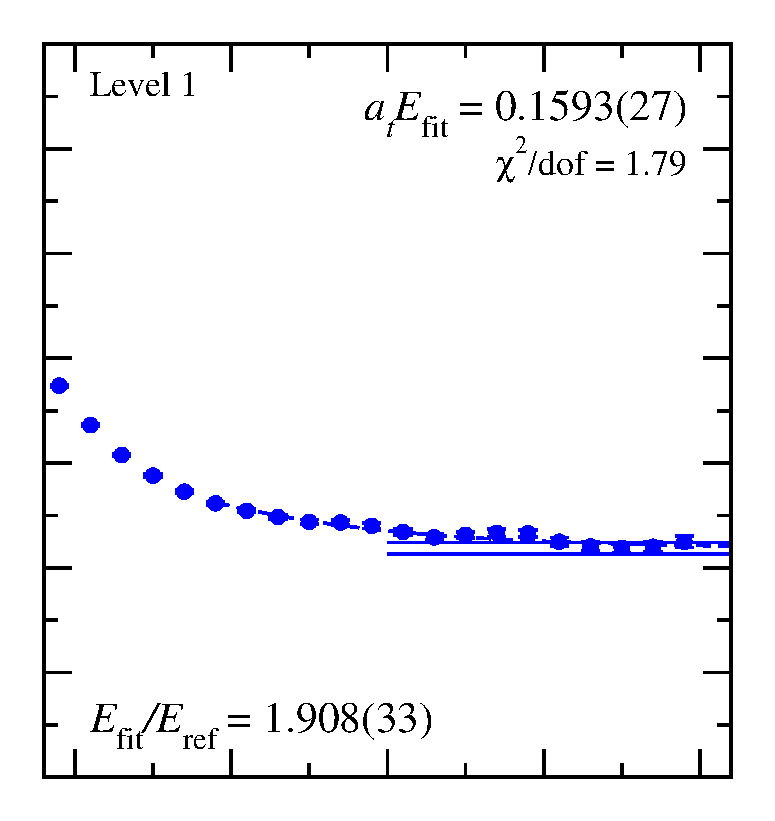
\includegraphics[width=0.28\textwidth]{figures/spectrum_a1g/no_tq/fits/fit_1.pdf}
  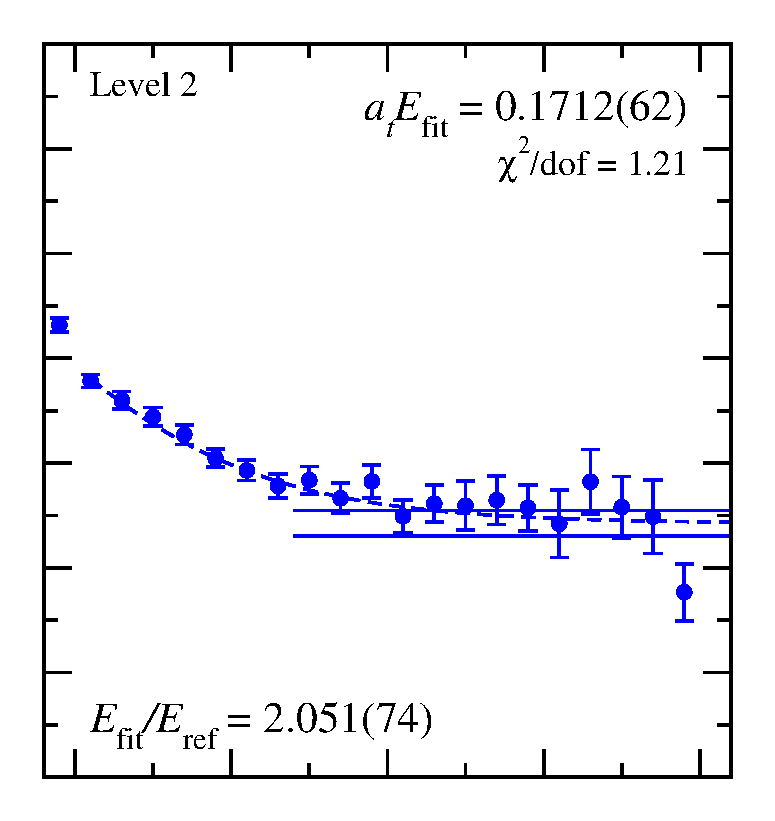
\includegraphics[width=0.28\textwidth]{figures/spectrum_a1g/no_tq/fits/fit_2.pdf}\\
  \raisebox{-.08cm}{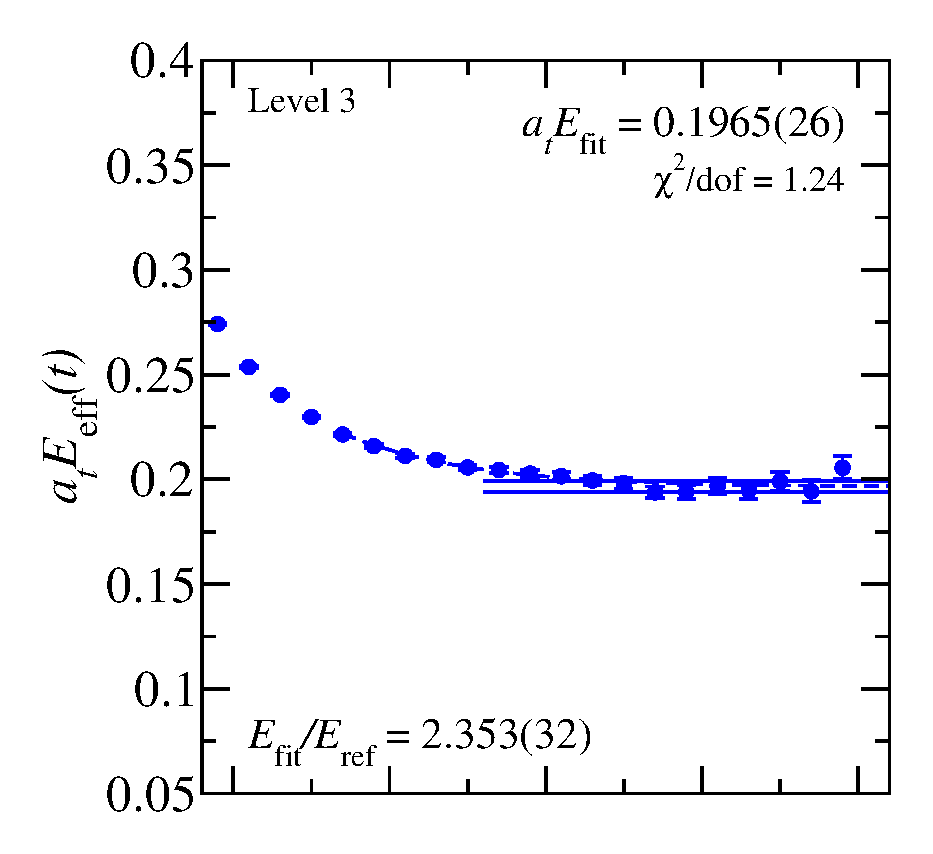
\includegraphics[width=0.336\textwidth]{figures/spectrum_a1g/no_tq/fits/fit_3.pdf}}
  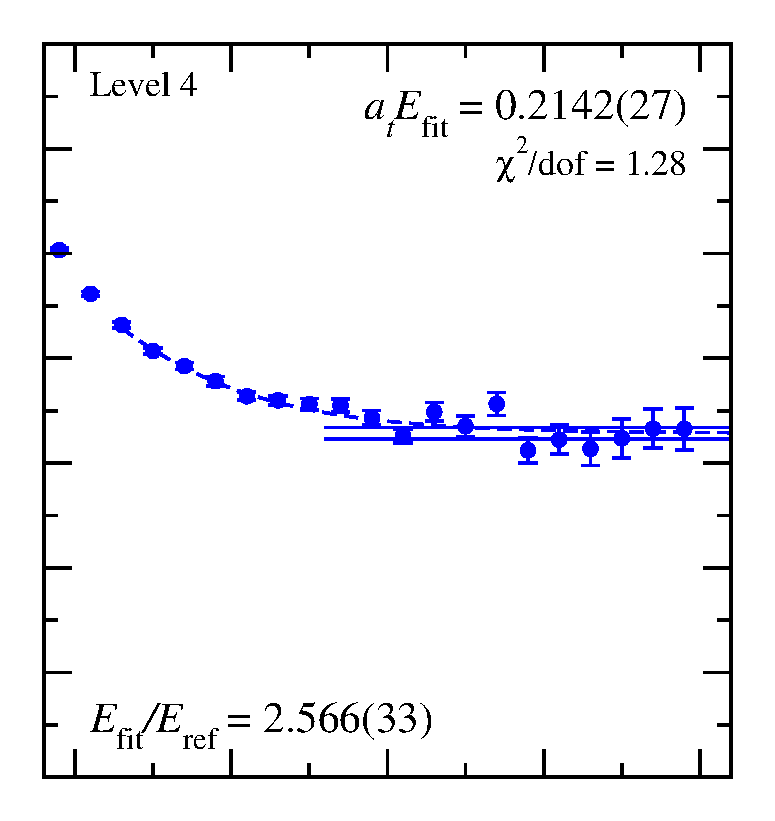
\includegraphics[width=0.28\textwidth]{figures/spectrum_a1g/no_tq/fits/fit_4.pdf}
  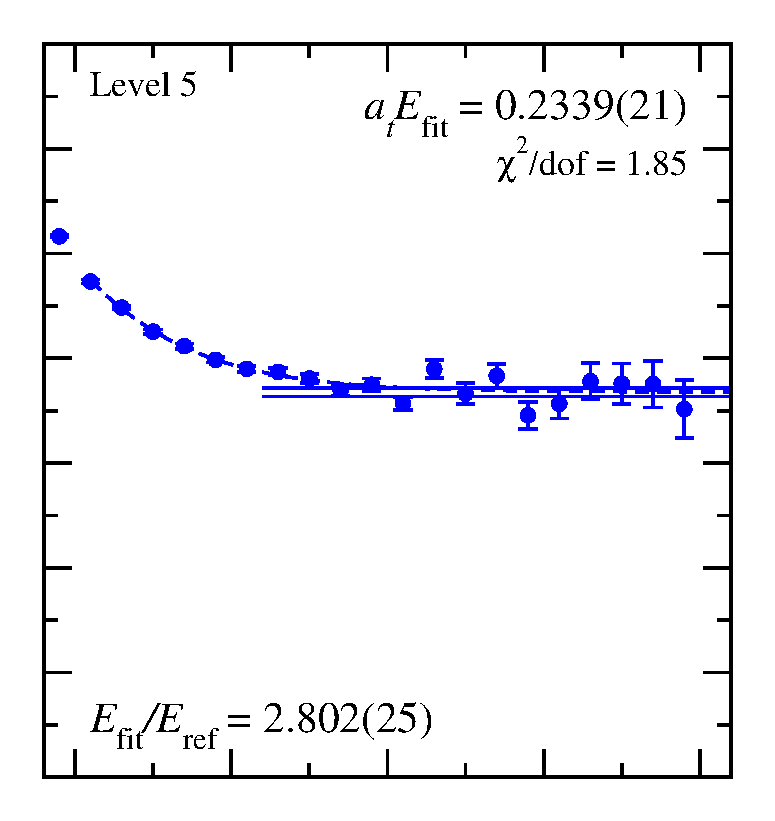
\includegraphics[width=0.28\textwidth]{figures/spectrum_a1g/no_tq/fits/fit_5.pdf}\\
  \raisebox{0.2in}{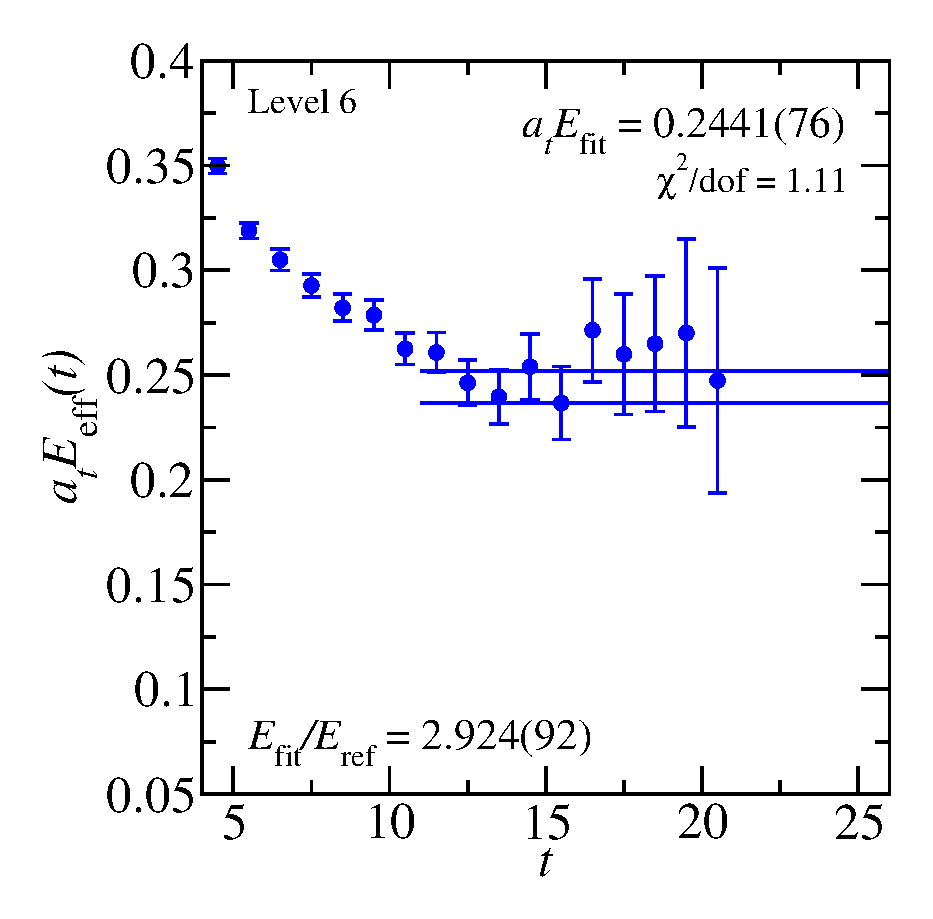
\includegraphics[width=0.336\textwidth]{figures/spectrum_a1g/no_tq/fits/fit_7.pdf}}
  \raisebox{0.2in}{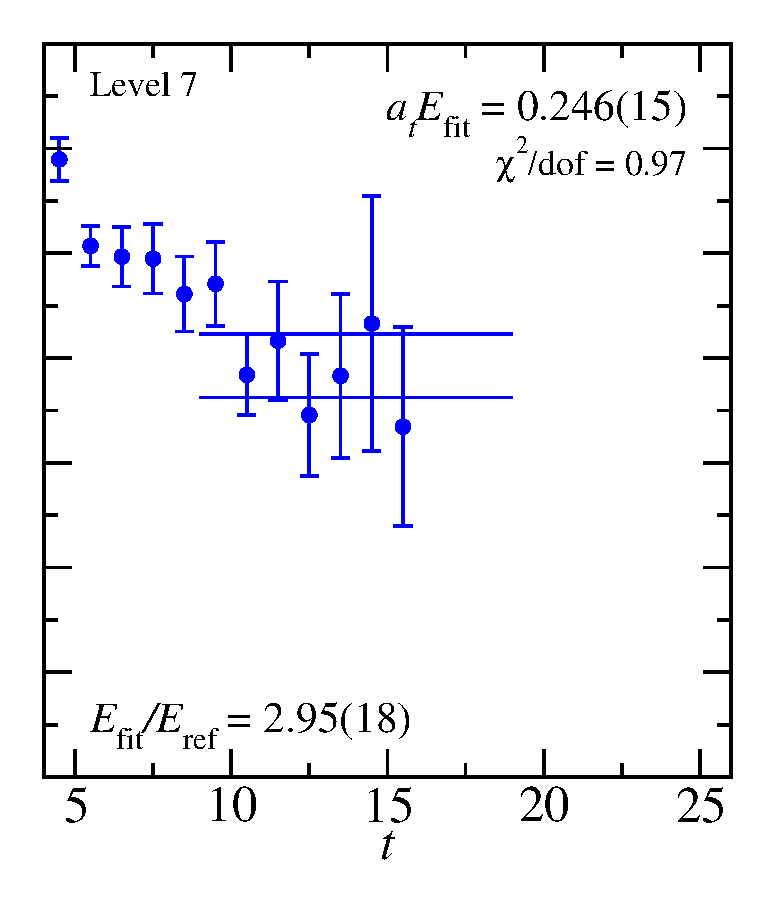
\includegraphics[width=0.28\textwidth]{figures/spectrum_a1g/no_tq/fits/fit_6.pdf}}
  \raisebox{0.2in}{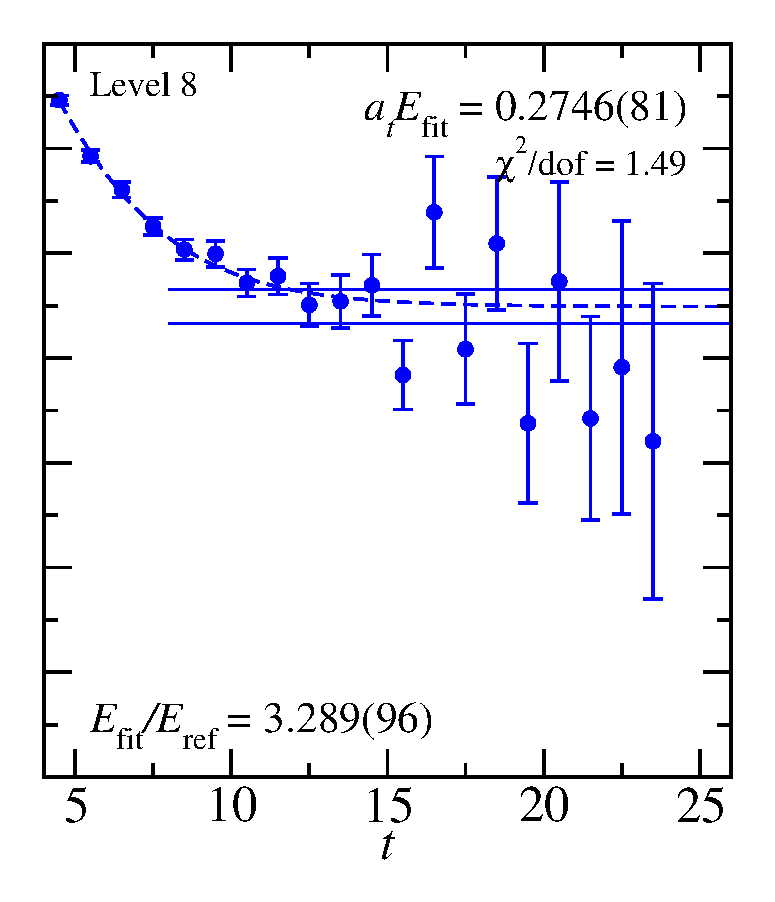
\includegraphics[width=0.28\textwidth]{figures/spectrum_a1g/no_tq/fits/fit_8.pdf}}
  \caption[Effective energies for the rotated $11\times 11$ correlator matrix in the $\kappa$ channel, using the operator basis given in Table~\ref{table:kappa_ops_no_tq}.]{Effective energies for the rotated $11\times 11$ correlator matrix in the $\kappa$ channel, using the operator basis given in Table~\ref{table:kappa_ops_no_tq}, which contains no tetraquark operators. Effective energy curves calculated from correlator fits are overlaid, and fit results are shown.}
  \label{fig:kappa_no_tq_grid}
\end{figure}

\begin{figure}
  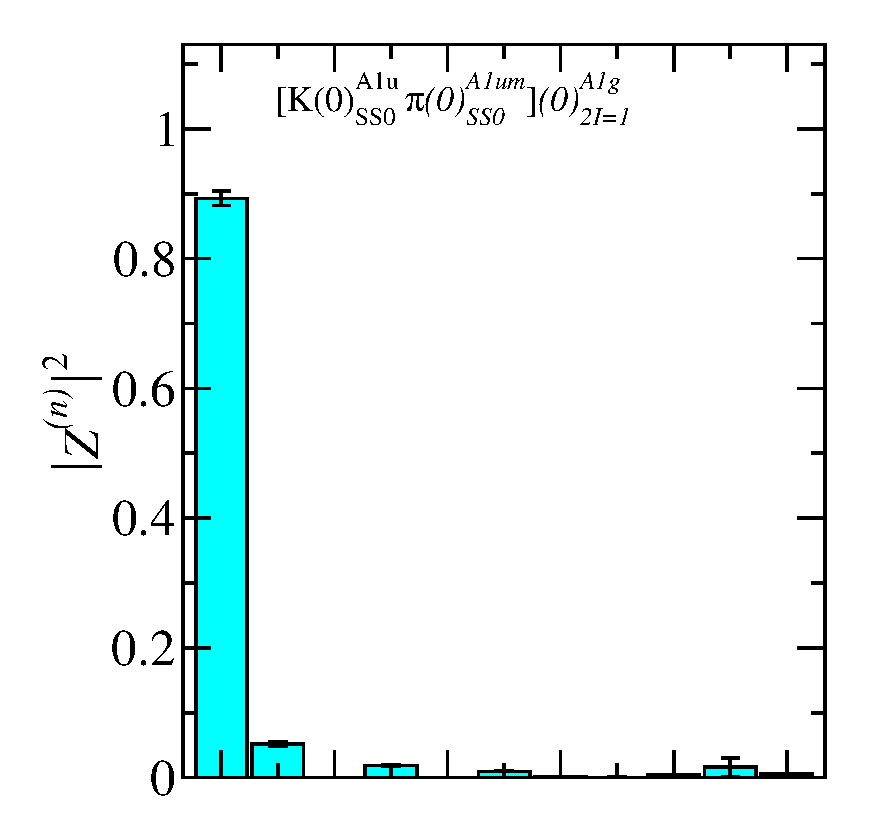
\includegraphics[width=0.304\textwidth]{figures/spectrum_a1g/no_tq/zfactors/zfactor_isodoublet_kaon_pion-A1g_1-P000-A1u-SS_0-P000-A1um-SS_0.pdf}
  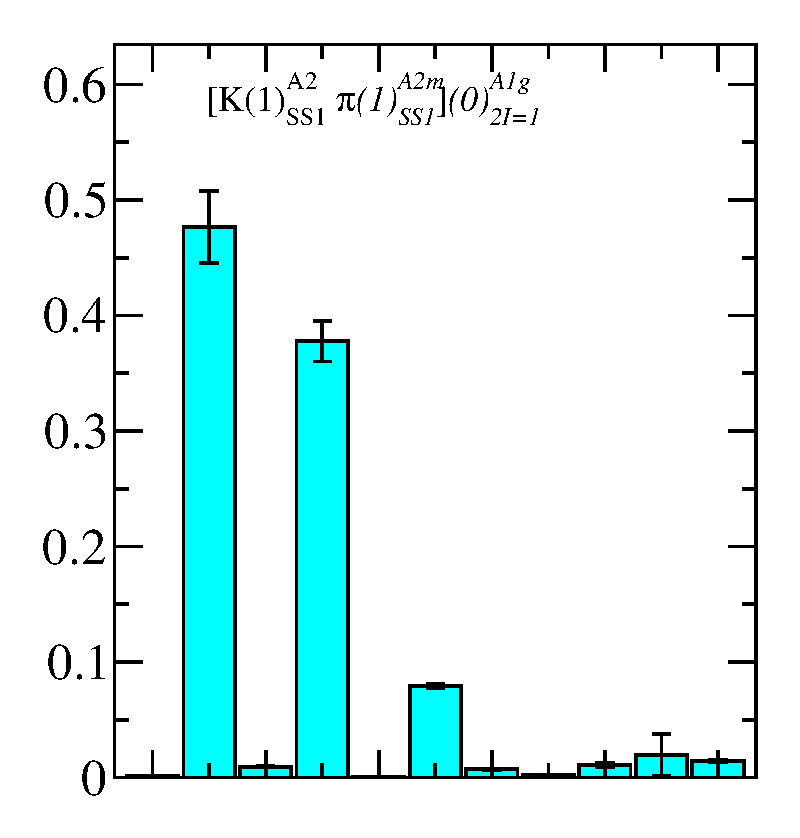
\includegraphics[width=0.28\textwidth]{figures/spectrum_a1g/no_tq/zfactors/zfactor_isodoublet_kaon_pion-A1g_1-P001-A2-SS_1-P00-1-A2m-SS_1.pdf}
  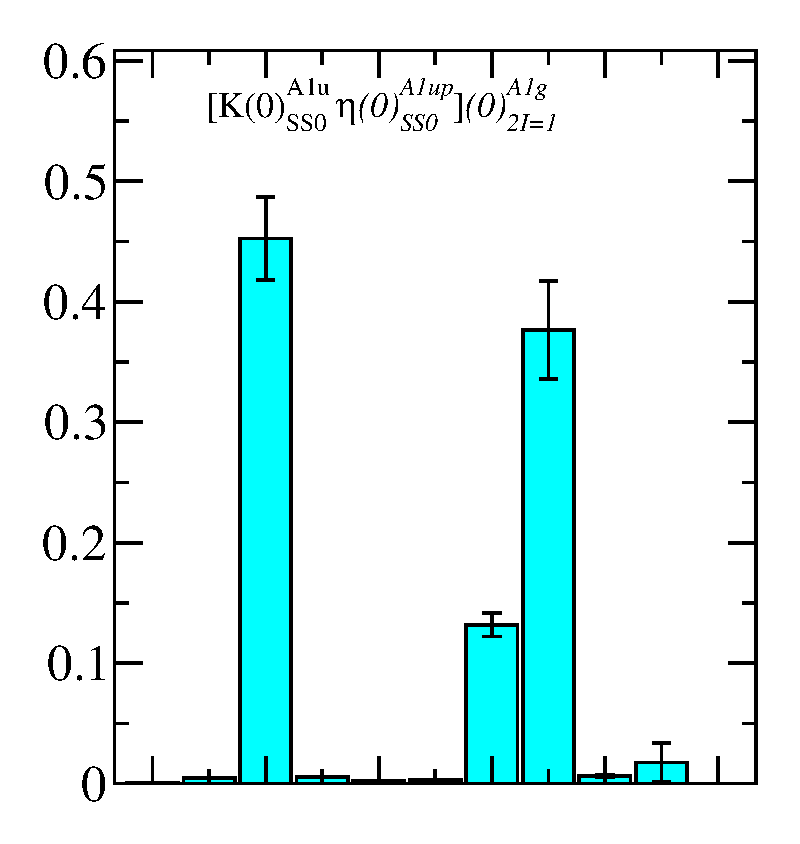
\includegraphics[width=0.28\textwidth]{figures/spectrum_a1g/no_tq/zfactors/zfactor_isodoublet_kaon_eta-A1g_1-P000-A1u-SS_0-P000-A1up-SS_0.pdf}\\
  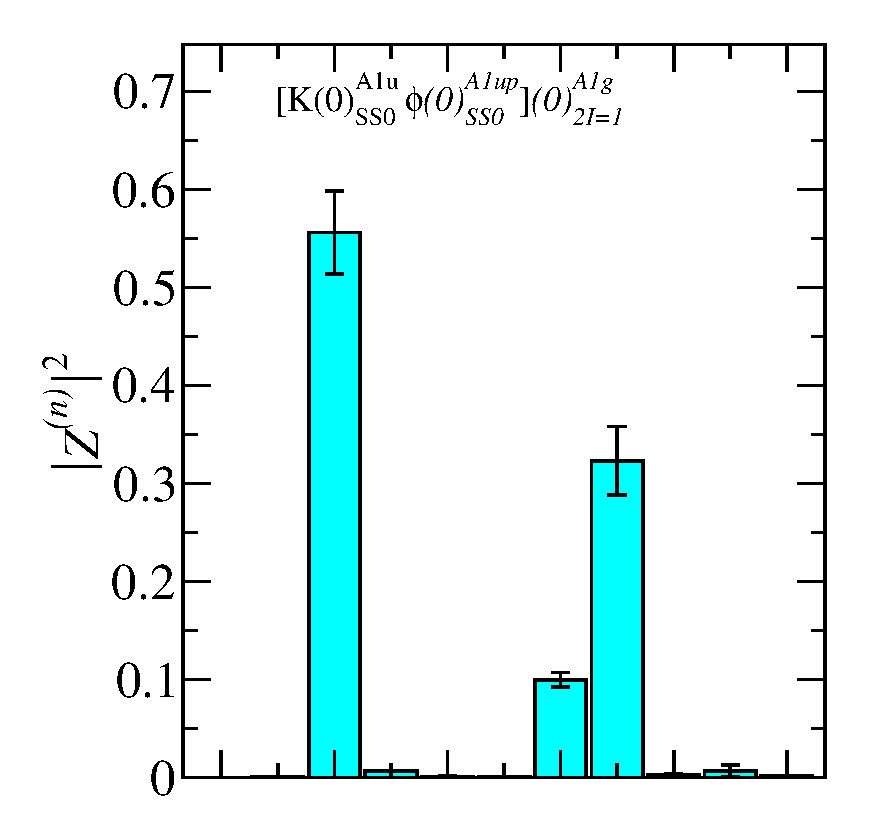
\includegraphics[width=0.304\textwidth]{figures/spectrum_a1g/no_tq/zfactors/zfactor_isodoublet_kaon_phi-A1g_1-P000-A1u-SS_0-P000-A1up-SS_0.pdf}
  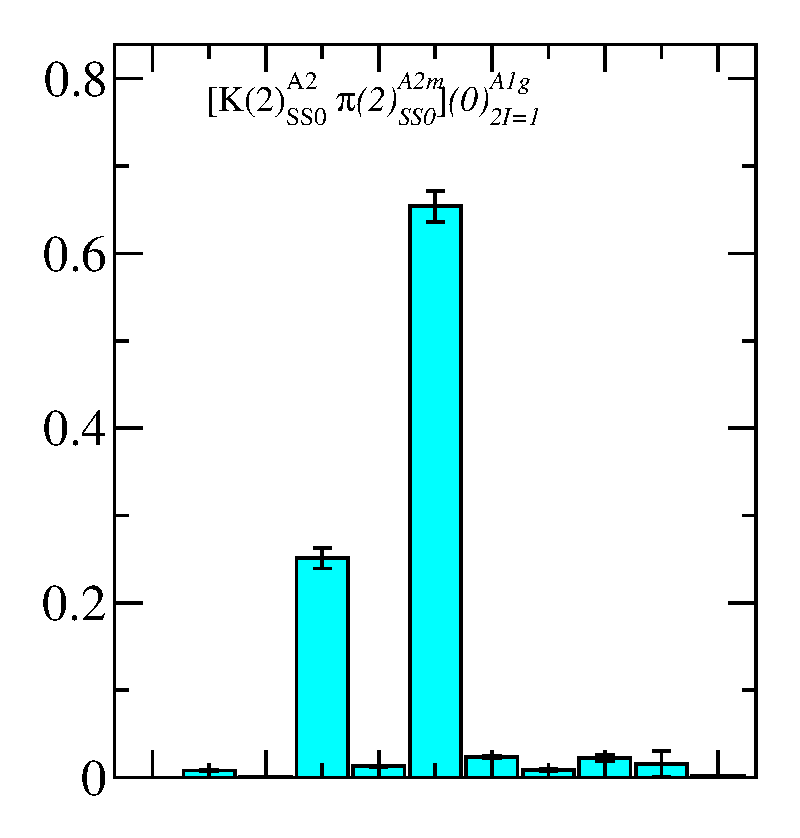
\includegraphics[width=0.28\textwidth]{figures/spectrum_a1g/no_tq/zfactors/zfactor_isodoublet_kaon_pion-A1g_1-P011-A2-SS_0-P0-1-1-A2m-SS_0.pdf}
  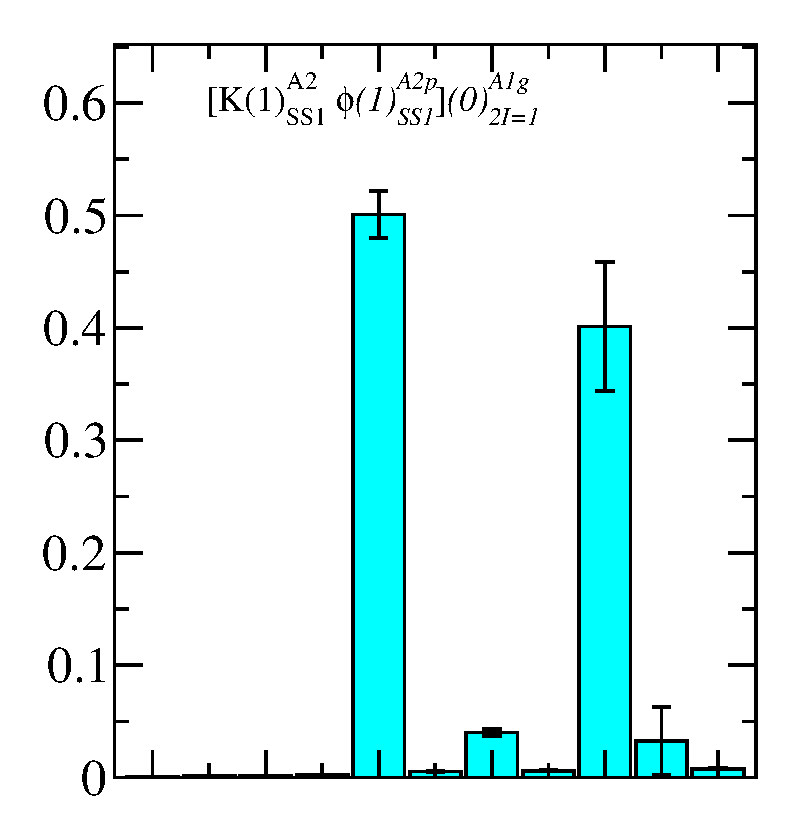
\includegraphics[width=0.28\textwidth]{figures/spectrum_a1g/no_tq/zfactors/zfactor_isodoublet_kaon_phi-A1g_1-P001-A2-SS_1-P00-1-A2p-SS_1.pdf}\\
  \raisebox{0.15in}{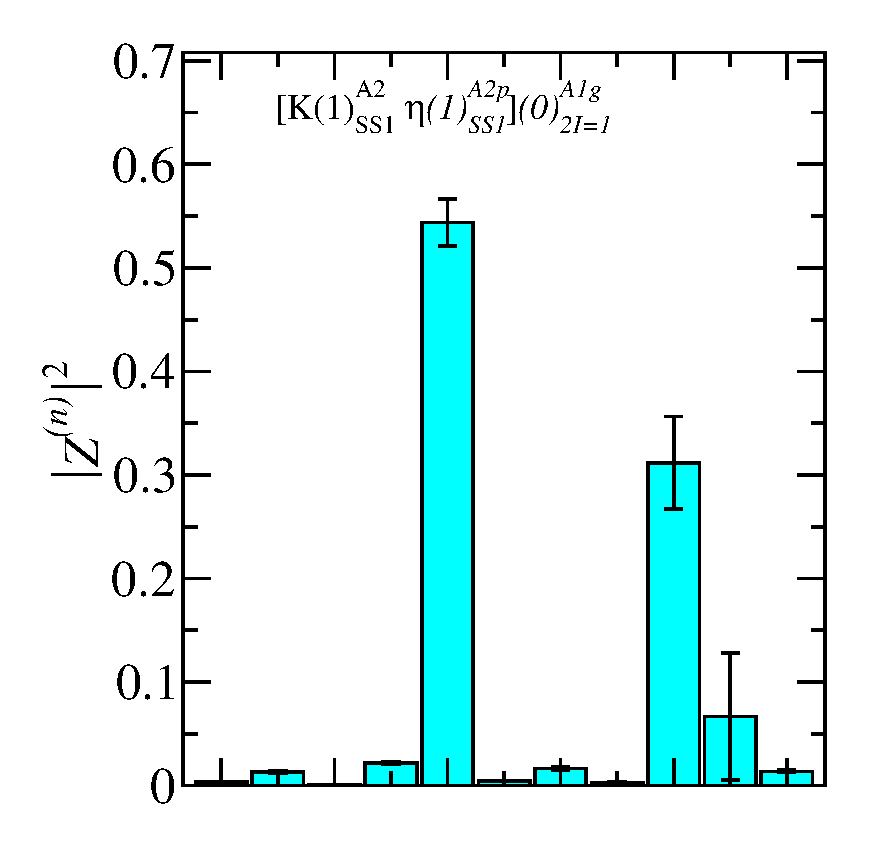
\includegraphics[width=0.304\textwidth]{figures/spectrum_a1g/no_tq/zfactors/zfactor_isodoublet_kaon_eta-A1g_1-P001-A2-SS_1-P00-1-A2p-SS_1.pdf}}
  \raisebox{0.15in}{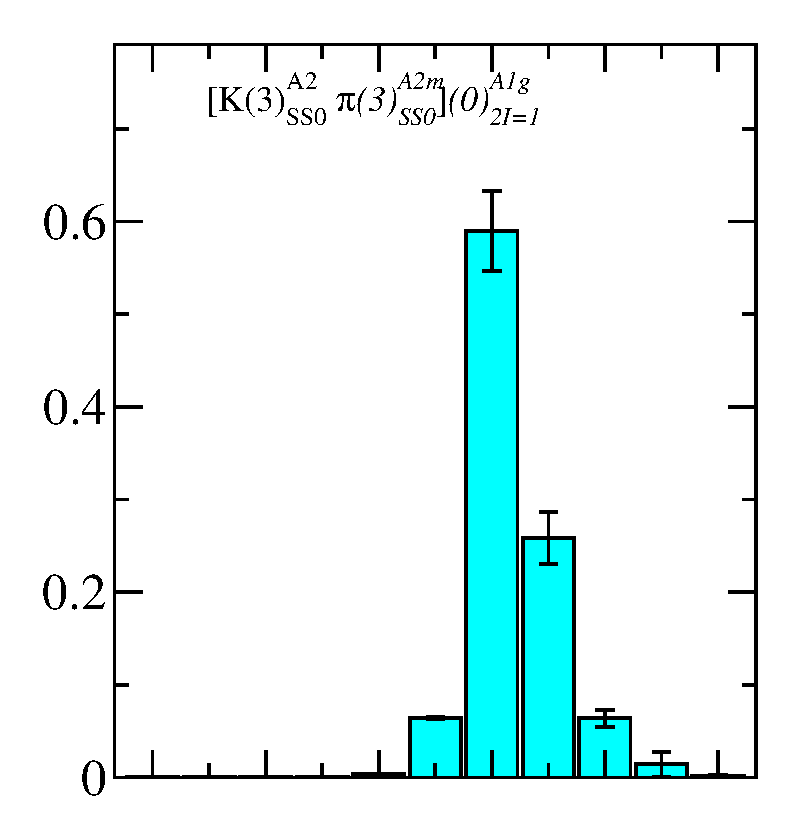
\includegraphics[width=0.28\textwidth]{figures/spectrum_a1g/no_tq/zfactors/zfactor_isodoublet_kaon_pion-A1g_1-P111-A2-SS_0-P-1-1-1-A2m-SS_0.pdf}}
  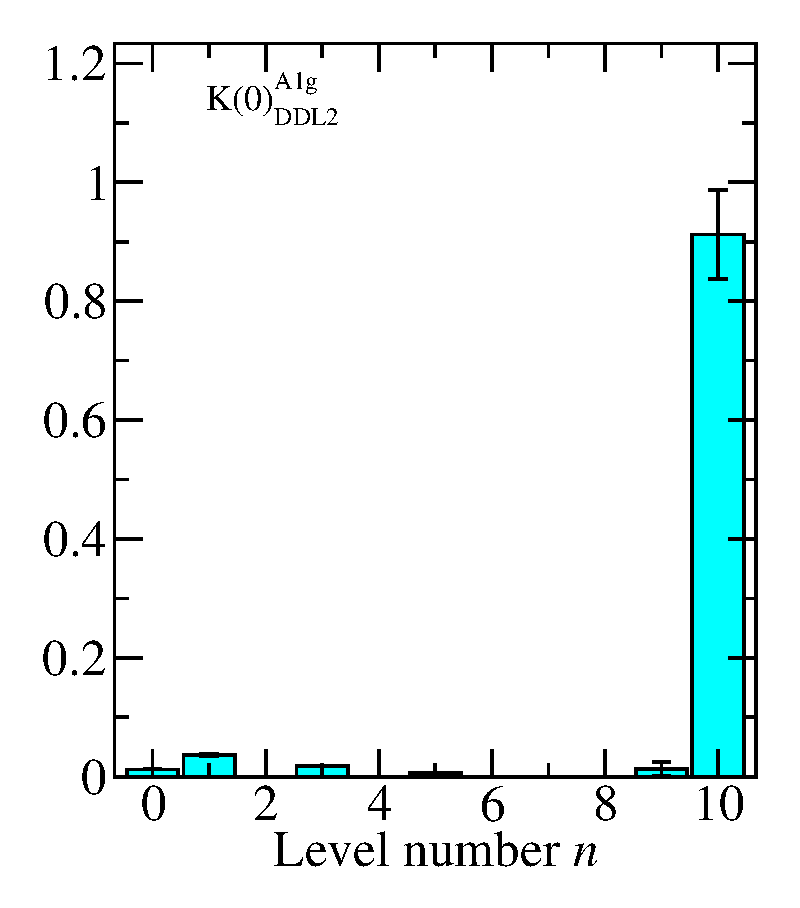
\includegraphics[width=0.28\textwidth]{figures/spectrum_a1g/no_tq/zfactors/zfactor_kaon-P000-A1g_1-DDL_2.pdf}\\
  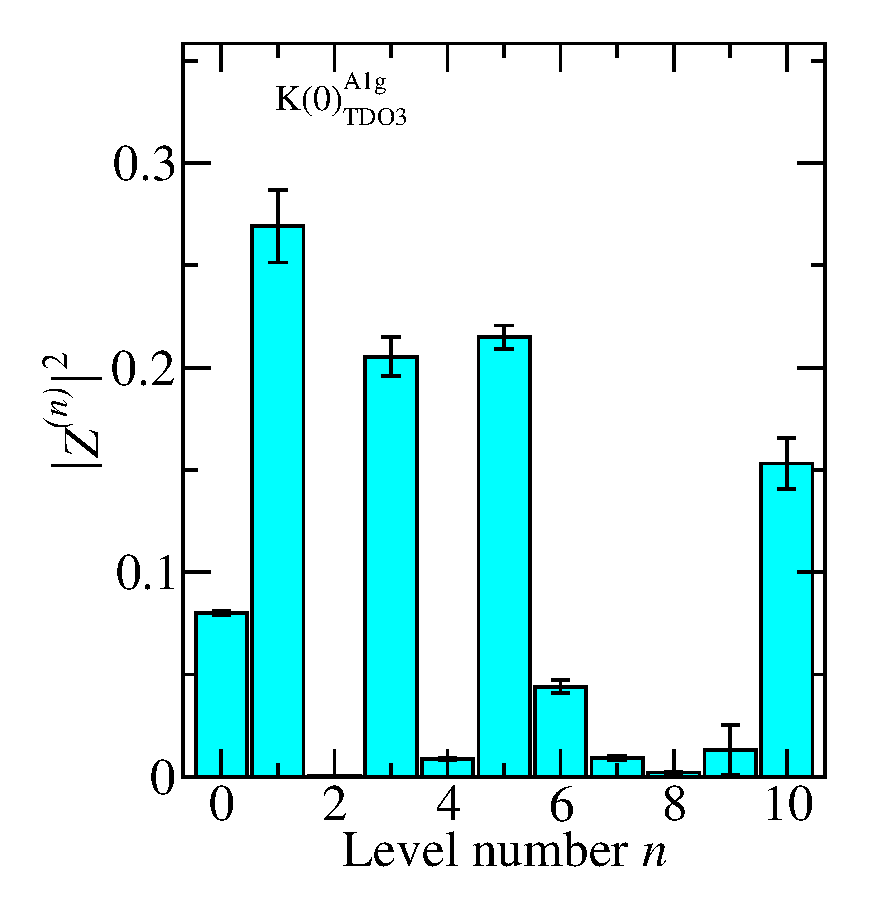
\includegraphics[width=0.304\textwidth]{figures/spectrum_a1g/no_tq/zfactors/zfactor_kaon-P000-A1g_1-TDO_3.pdf}
  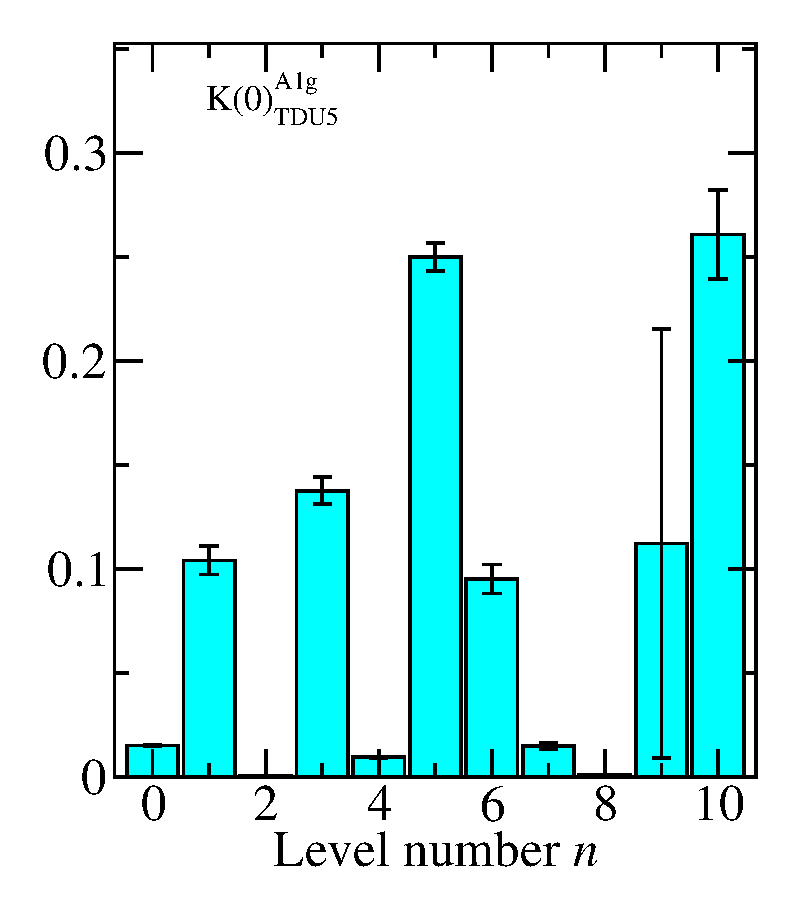
\includegraphics[width=0.28\textwidth]{figures/spectrum_a1g/no_tq/zfactors/zfactor_kaon-P000-A1g_1-TDU_5.pdf}
  \caption{Overlap factors for the operators used in the rotated $11\times 11$ correlator matrix in the $\kappa$ channel, using the operator basis given in Table~\ref{table:kappa_ops_no_tq}, which contains no tetraquark operators.}
  \label{fig:kappa_no_tq_zfactors}
\end{figure}

\begin{table}
  \centering
  \begin{tabular}{c|c|c|c|c}
    $E / E_K$ & $a_t E$ & Fit model & $(t_{\mathrm{min}}, {t_\mathrm{max}})$ & $\chi^2 / \rm{d.o.f.}$\\
    \hline
    1.4684(64)&0.12259(53)&2{-}exp&$(7, 26)$&0.58\\
1.908(33)&0.1593(27)&2{-}exp&$(8, 26)$&1.79\\%
2.051(74)&0.1712(62)&2{-}exp&$(4, 26)$&1.21\\
2.353(32)&0.1965(26)&2{-}exp&$(7, 26)$&1.24\\
2.566(33)&0.2142(27)&2{-}exp&$(5, 26)$&1.28\\
2.802(25)&0.2339(21)&2{-}exp&$(4, 26)$&1.85\\
2.924(92)&0.2441(76)&1{-}exp&$(11, 26)$&1.11\\
2.95(18)&0.246(15)&1{-}exp&$(9, 19)$&0.97\\
3.289(96)&0.2746(81)&2{-}exp&$(3, 26)$&1.49
  \end{tabular}
  \caption{Fit details for the estimate of the spectrum obtained in the $\kappa$ channel using the operator basis given in Table~\ref{table:kappa_ops_no_tq}, which contains no tetraquark operators.}
  \label{table:kappa_no_tq_spectrum}
\end{table}

\begin{figure}
  \raisebox{-.08cm}{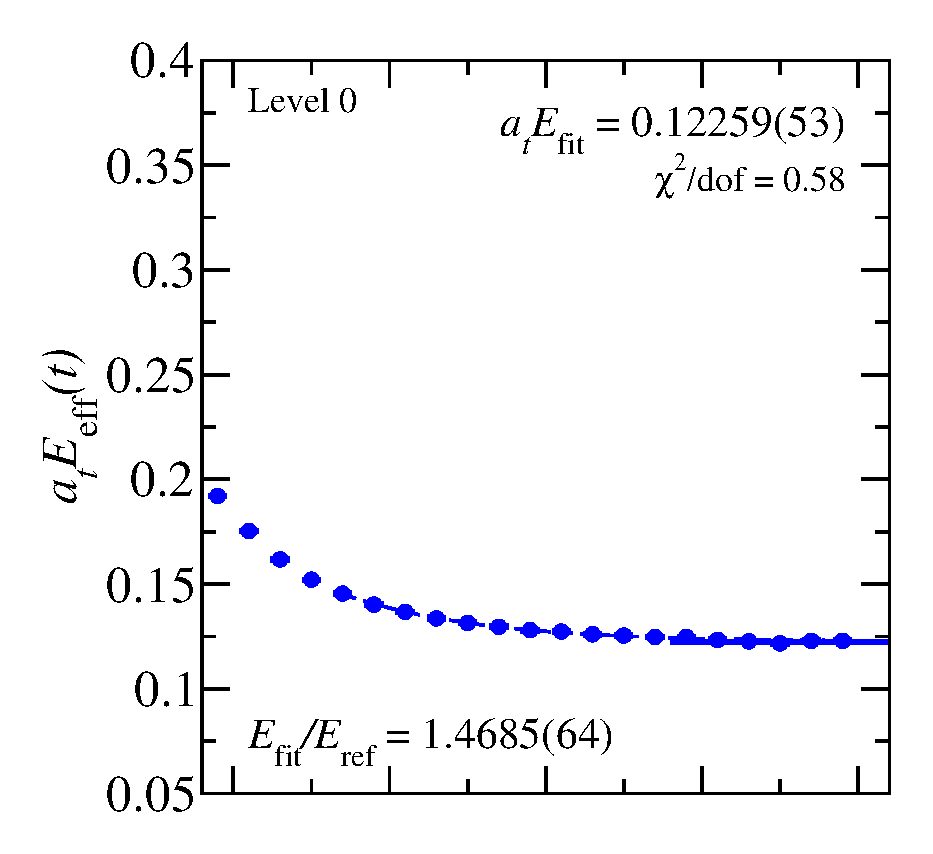
\includegraphics[width=0.336\textwidth]{figures/spectrum_a1g/with_tq/fits/fit_0.pdf}}
  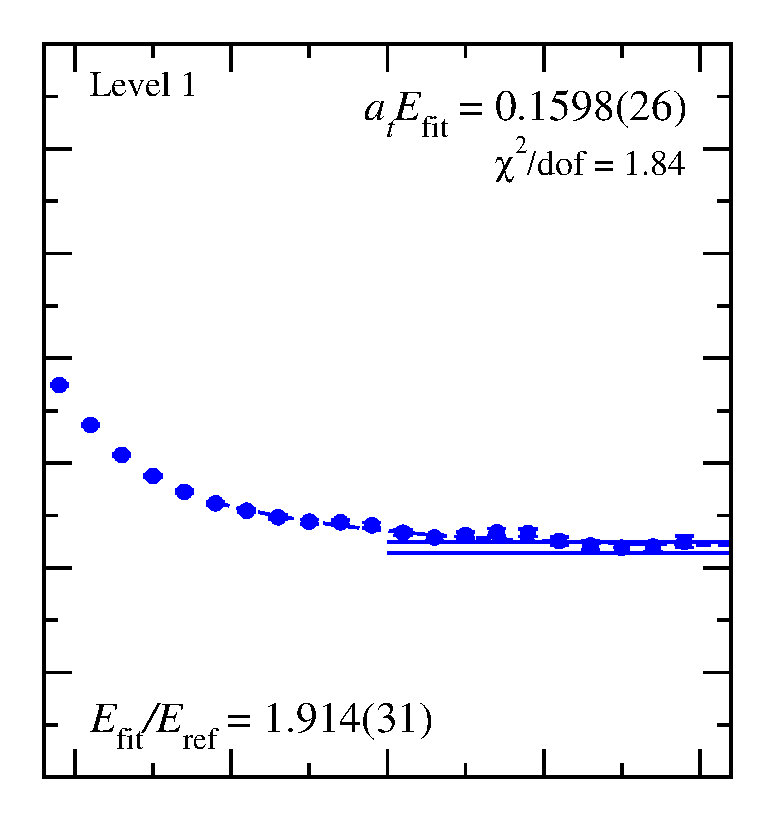
\includegraphics[width=0.28\textwidth]{figures/spectrum_a1g/with_tq/fits/fit_1.pdf}
  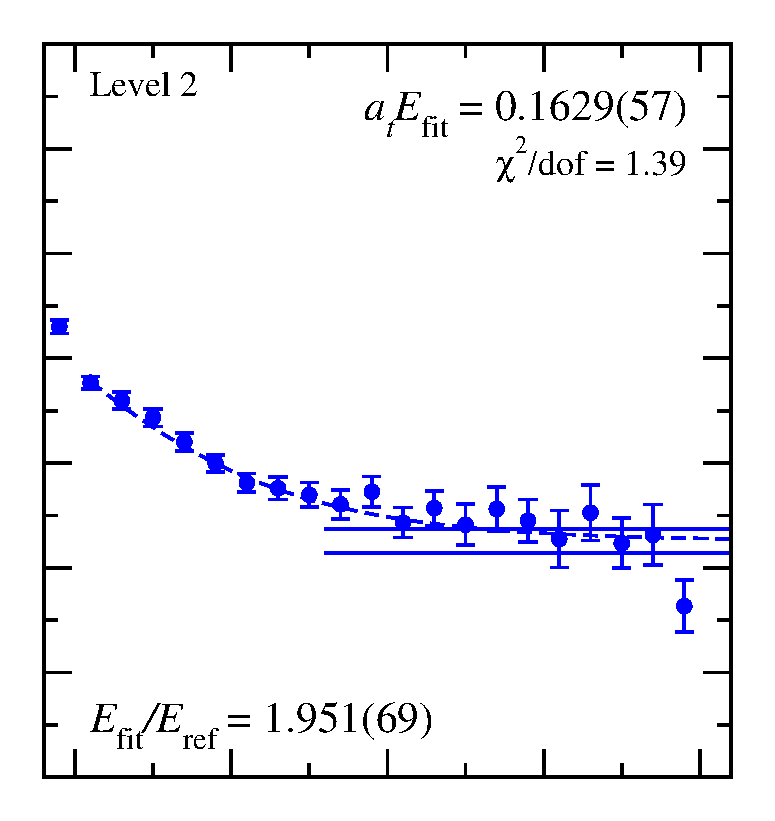
\includegraphics[width=0.28\textwidth]{figures/spectrum_a1g/with_tq/fits/fit_2.pdf}\\
  \raisebox{-.08cm}{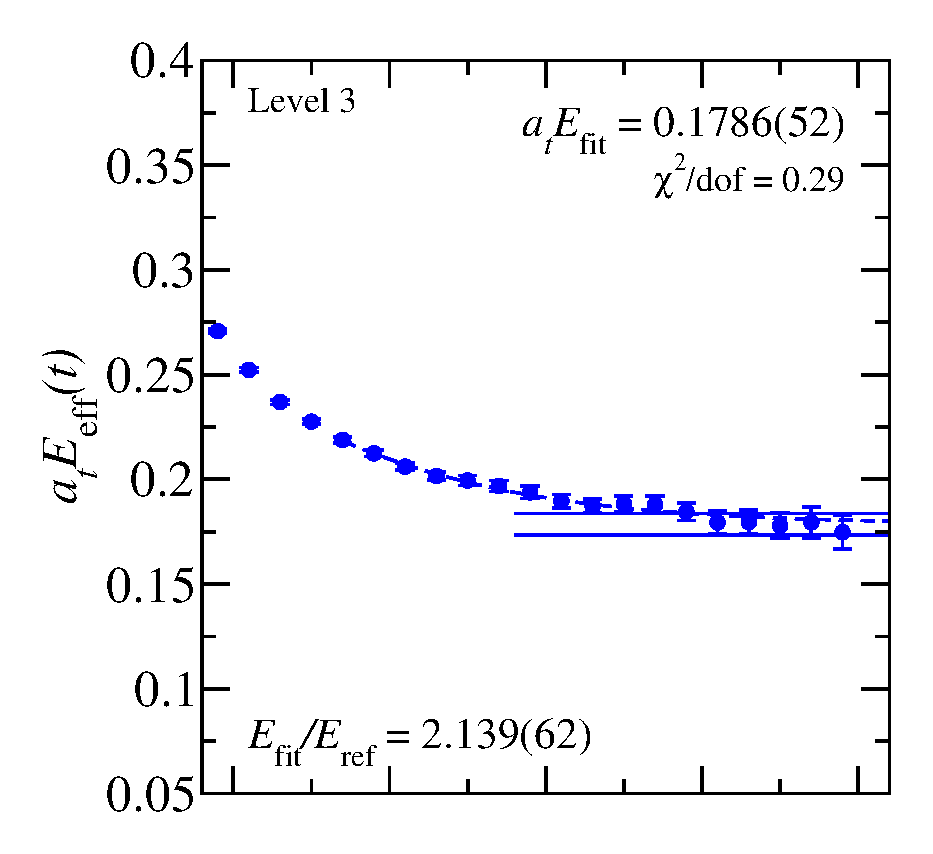
\includegraphics[width=0.336\textwidth]{figures/spectrum_a1g/with_tq/fits/fit_3.pdf}}
  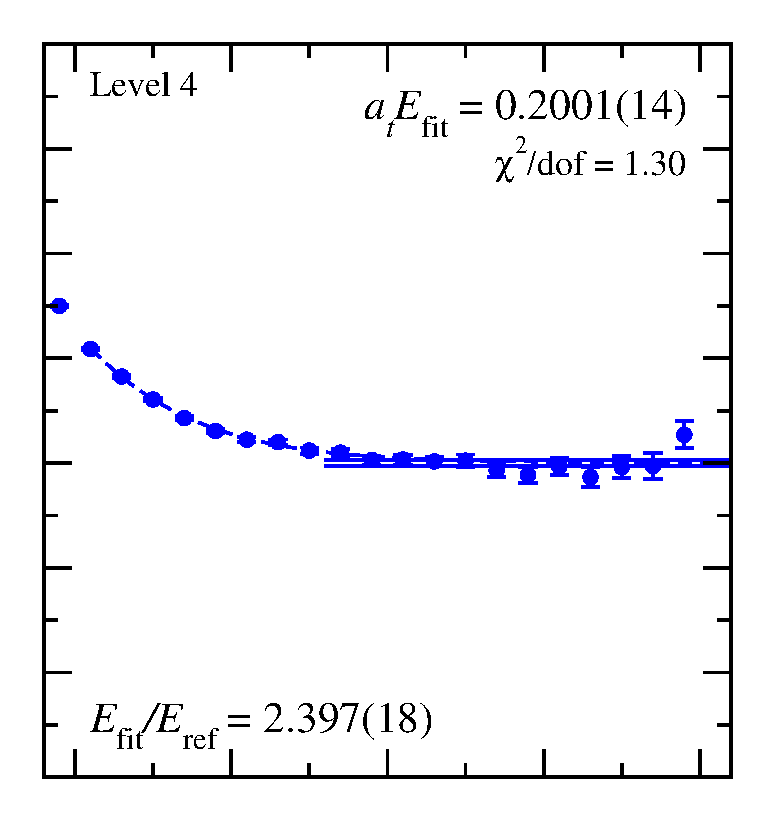
\includegraphics[width=0.28\textwidth]{figures/spectrum_a1g/with_tq/fits/fit_4.pdf}
  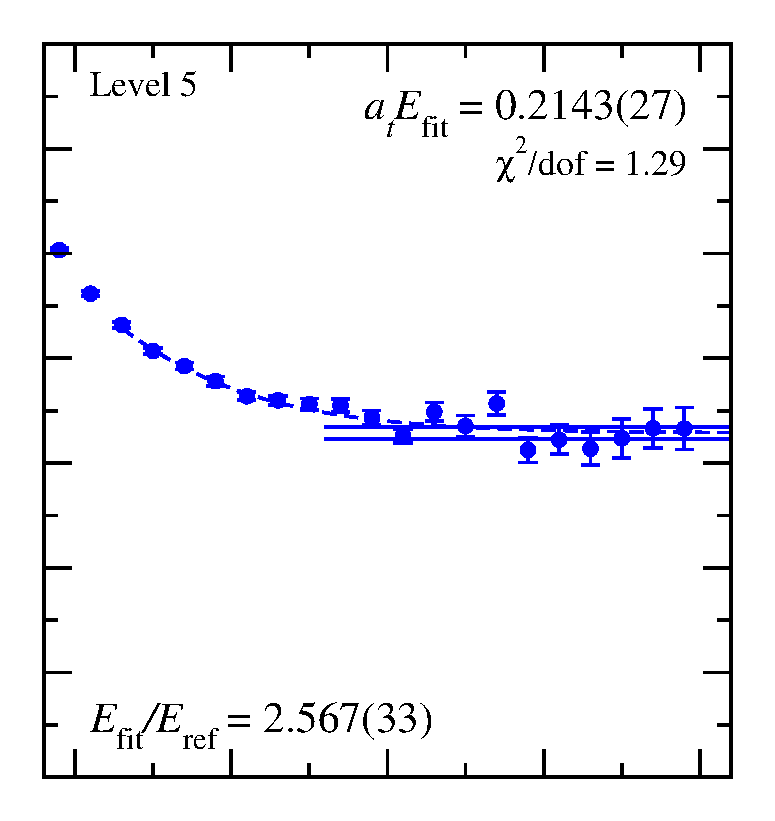
\includegraphics[width=0.28\textwidth]{figures/spectrum_a1g/with_tq/fits/fit_5.pdf}\\
  \raisebox{0.15in}{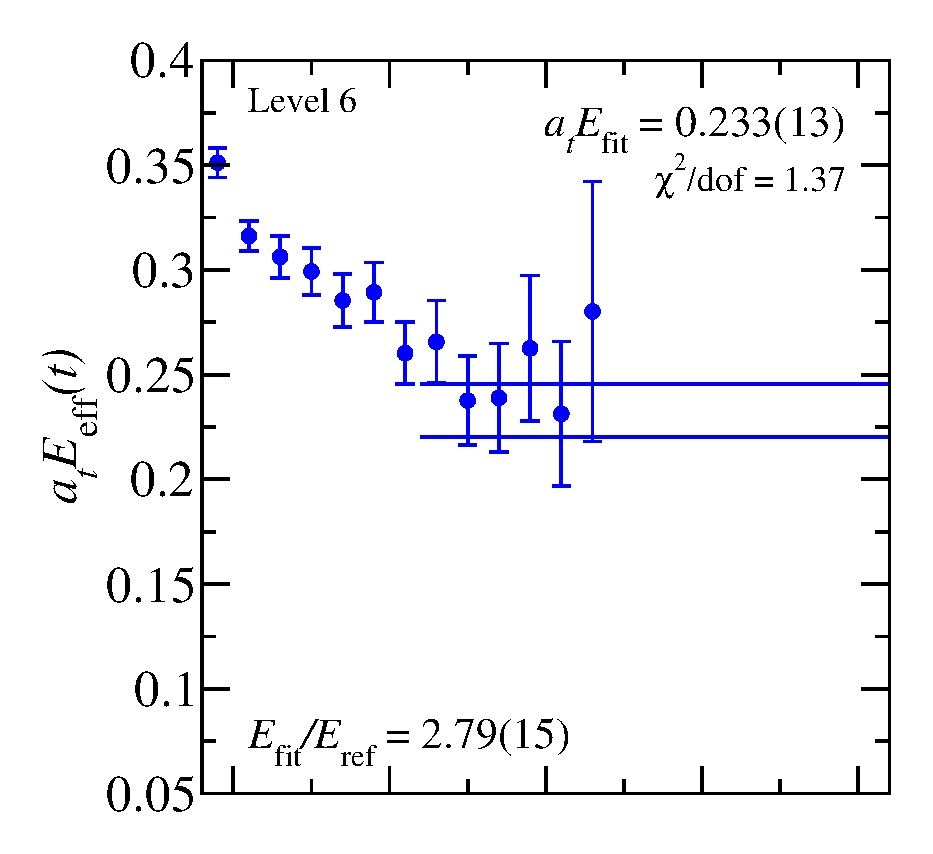
\includegraphics[width=0.338\textwidth]{figures/spectrum_a1g/with_tq/fits/fit_8.pdf}}
  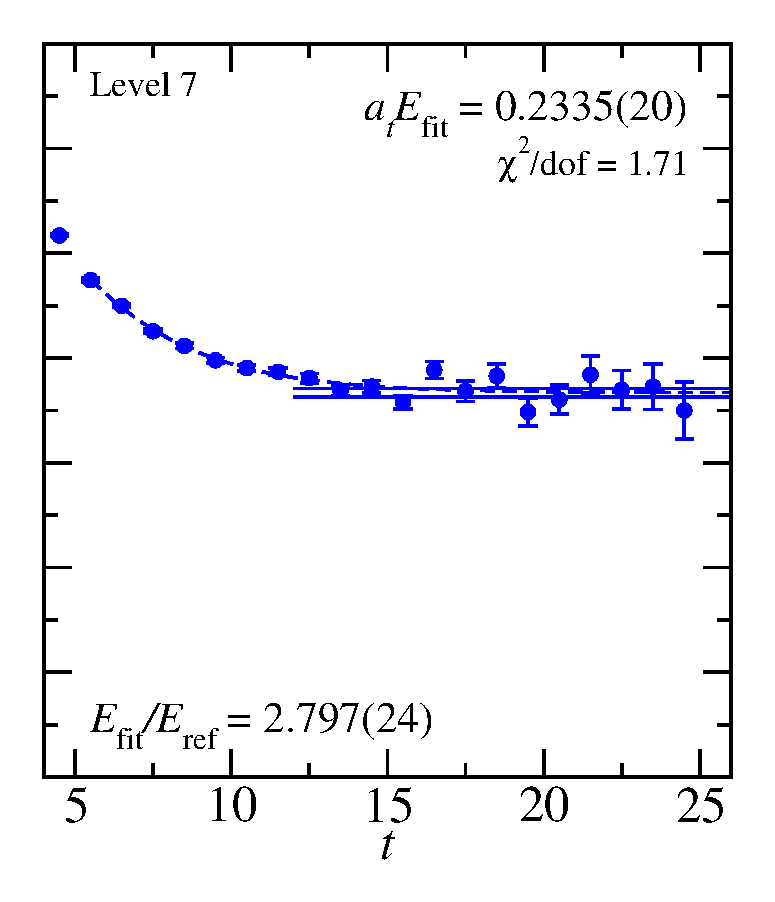
\includegraphics[width=0.28\textwidth]{figures/spectrum_a1g/with_tq/fits/fit_6.pdf}
  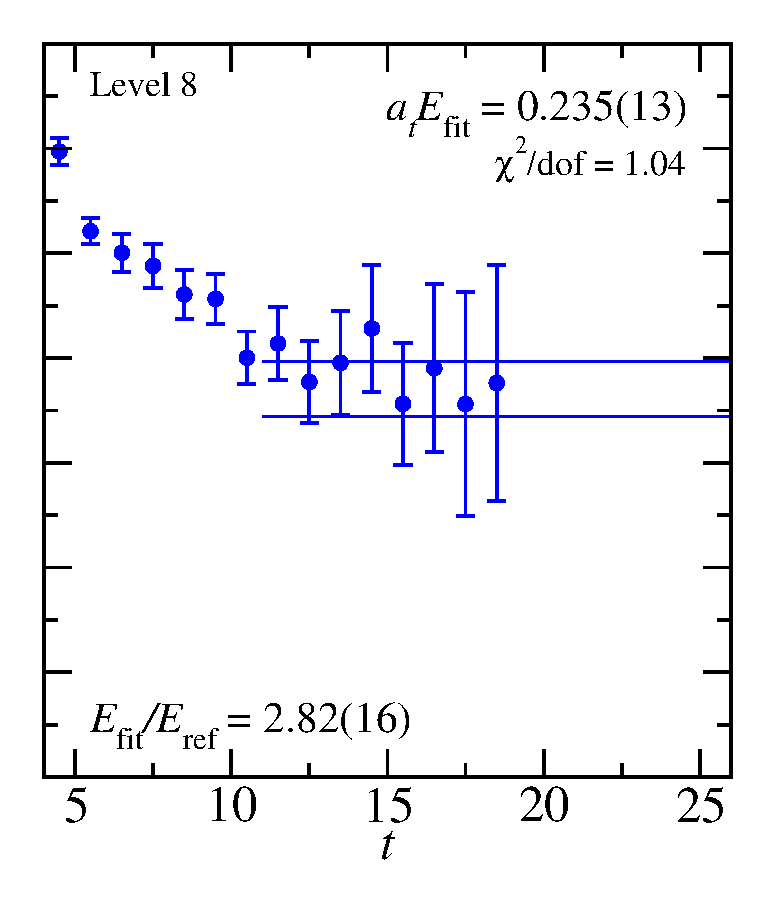
\includegraphics[width=0.28\textwidth]{figures/spectrum_a1g/with_tq/fits/fit_7.pdf}\\[-0.4cm]
  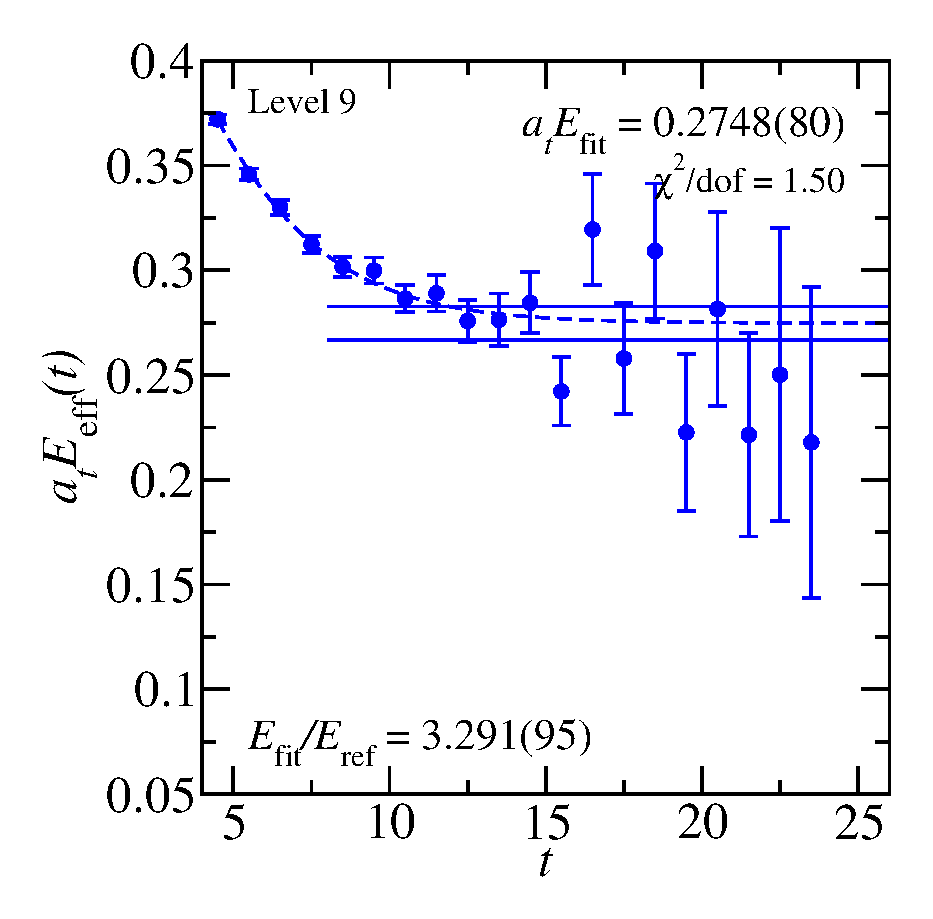
\includegraphics[width=0.336\textwidth]{figures/spectrum_a1g/with_tq/fits/fit_9.pdf}
  \caption[Effective energies for the rotated $12\times 12$ correlator matrix in the $\kappa$ channel, using the operator basis given in Table~\ref{table:kappa_ops_no_tq}, but with the addition of one tetraquark operator.]{Effective energies for the rotated $12\times 12$ correlator matrix in the $\kappa$ channel, using the operator basis given in Table~\ref{table:kappa_ops_no_tq}, but with the addition of one tetraquark operator. Effective energy curves calculated from correlator fits are overlaid, and fit results are shown.}
  \label{fig:kappa_with_tq_grid}
\end{figure}

\begin{figure}
  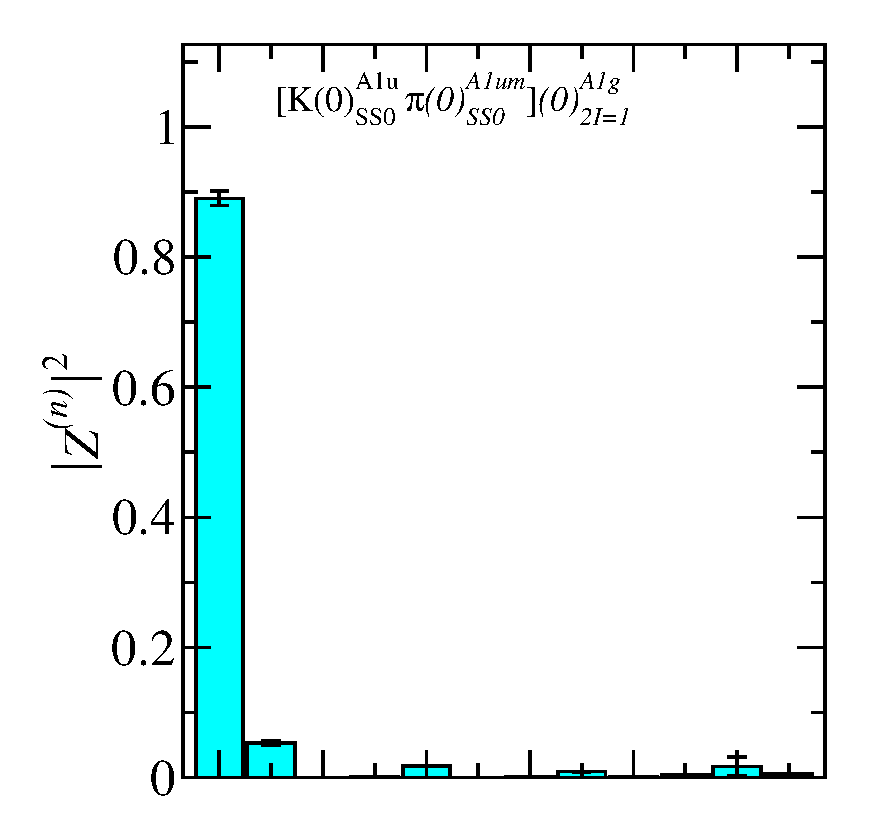
\includegraphics[width=0.304\textwidth]{figures/spectrum_a1g/with_tq/zfactors/zfactor_isodoublet_kaon_pion-A1g_1-P000-A1u-SS_0-P000-A1um-SS_0.pdf}
  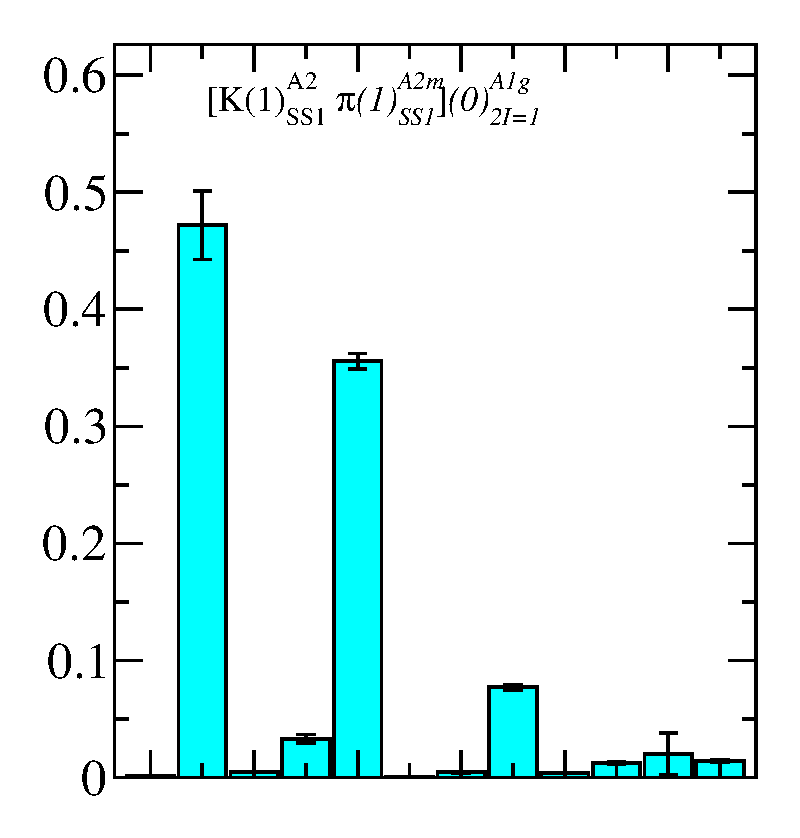
\includegraphics[width=0.28\textwidth]{figures/spectrum_a1g/with_tq/zfactors/zfactor_isodoublet_kaon_pion-A1g_1-P001-A2-SS_1-P00-1-A2m-SS_1.pdf}
  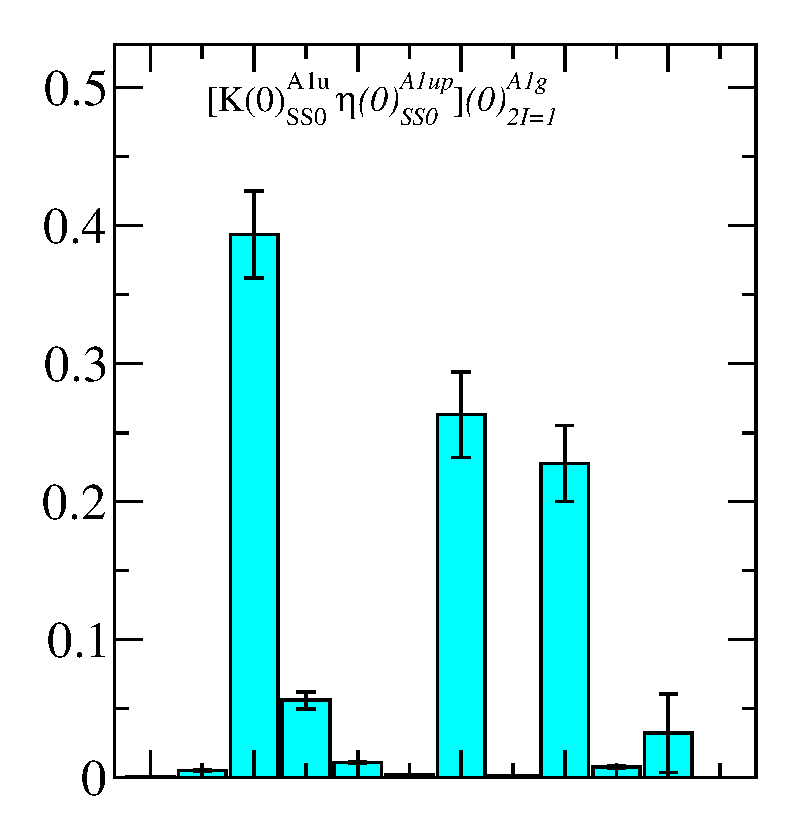
\includegraphics[width=0.28\textwidth]{figures/spectrum_a1g/with_tq/zfactors/zfactor_isodoublet_kaon_eta-A1g_1-P000-A1u-SS_0-P000-A1up-SS_0.pdf}\\
  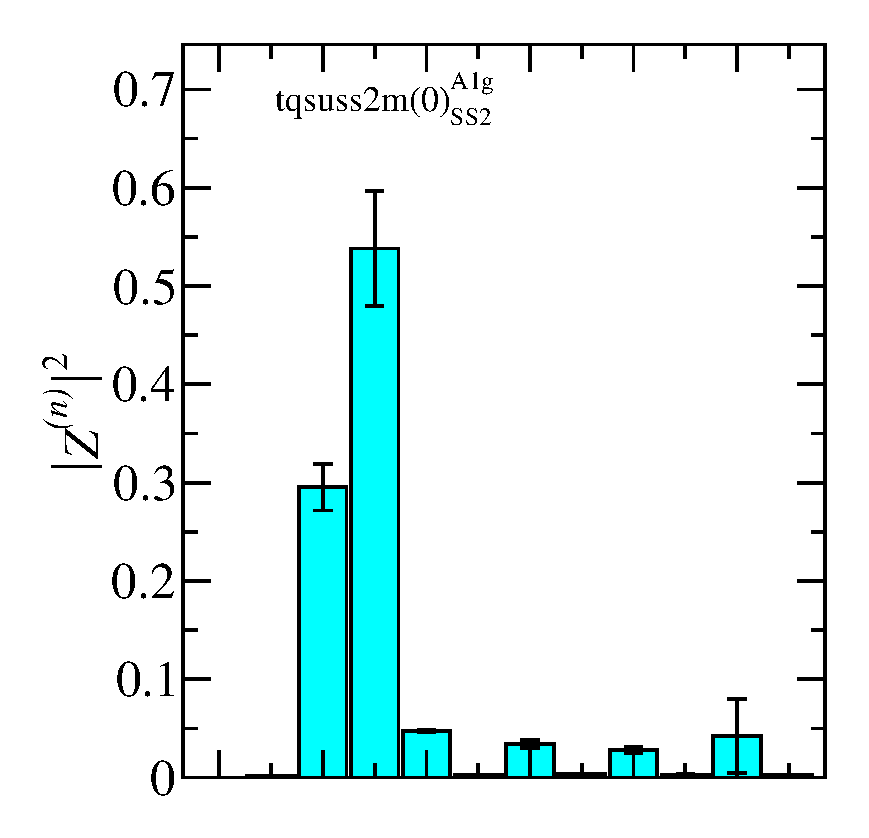
\includegraphics[width=0.304\textwidth]{figures/spectrum_a1g/with_tq/zfactors/zfactor_tqsuss2m-P000-A1g_1-SS_2.pdf}
  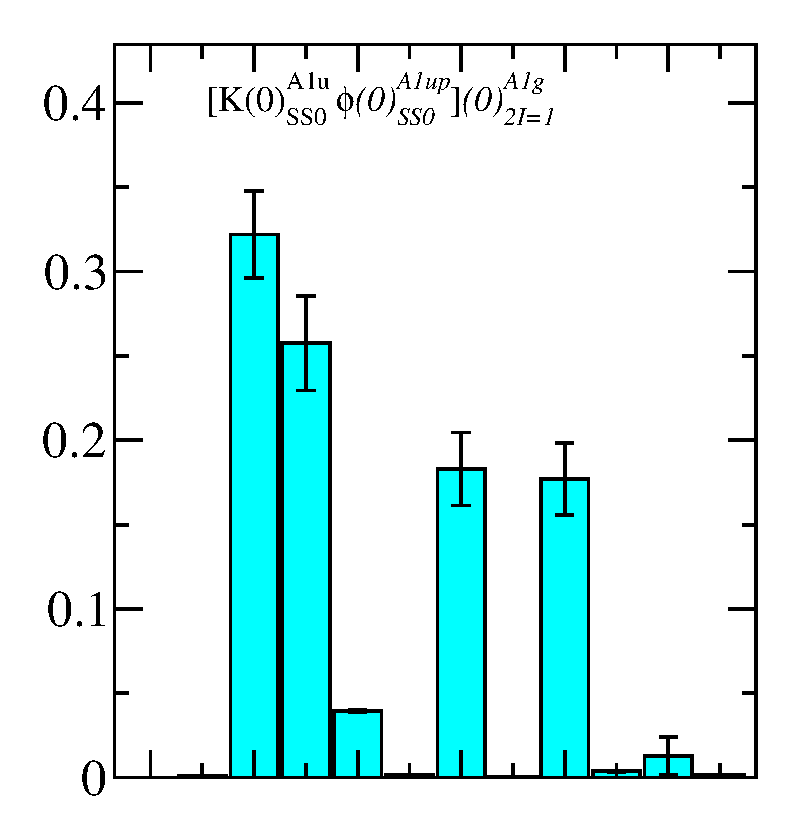
\includegraphics[width=0.28\textwidth]{figures/spectrum_a1g/with_tq/zfactors/zfactor_isodoublet_kaon_phi-A1g_1-P000-A1u-SS_0-P000-A1up-SS_0.pdf}
  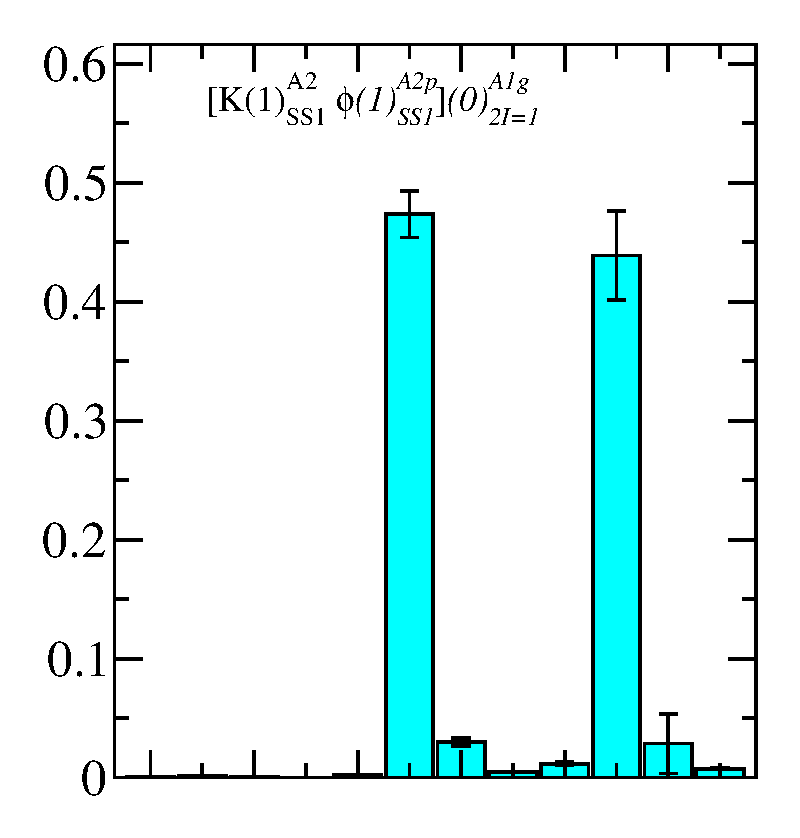
\includegraphics[width=0.28\textwidth]{figures/spectrum_a1g/with_tq/zfactors/zfactor_isodoublet_kaon_phi-A1g_1-P001-A2-SS_1-P00-1-A2p-SS_1.pdf}\\
  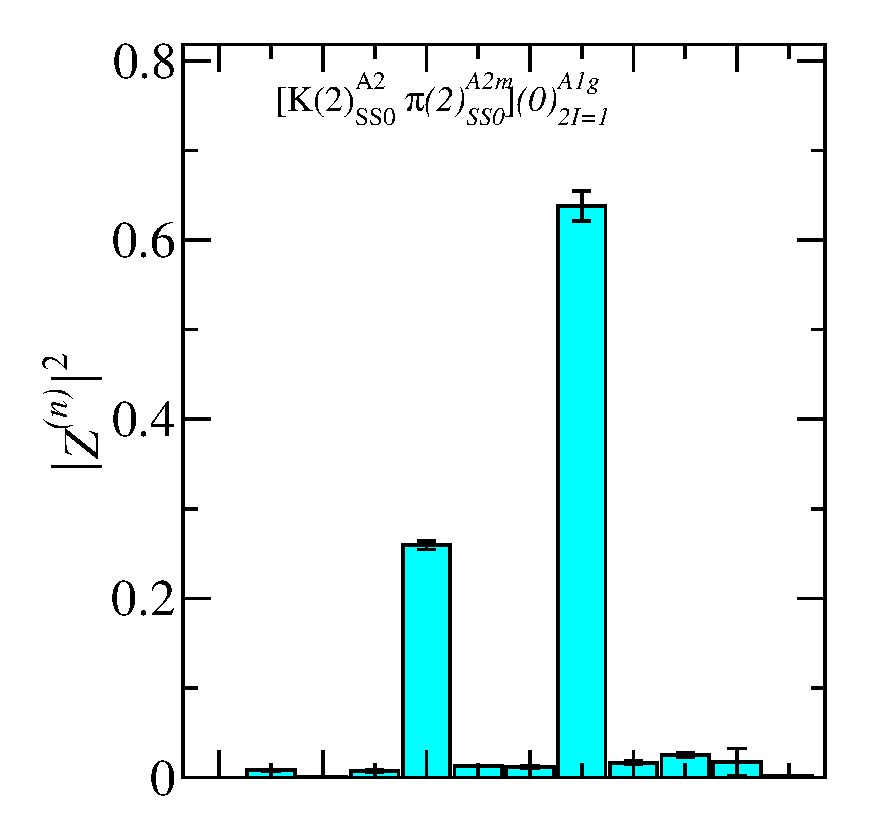
\includegraphics[width=0.304\textwidth]{figures/spectrum_a1g/with_tq/zfactors/zfactor_isodoublet_kaon_pion-A1g_1-P011-A2-SS_0-P0-1-1-A2m-SS_0.pdf}
  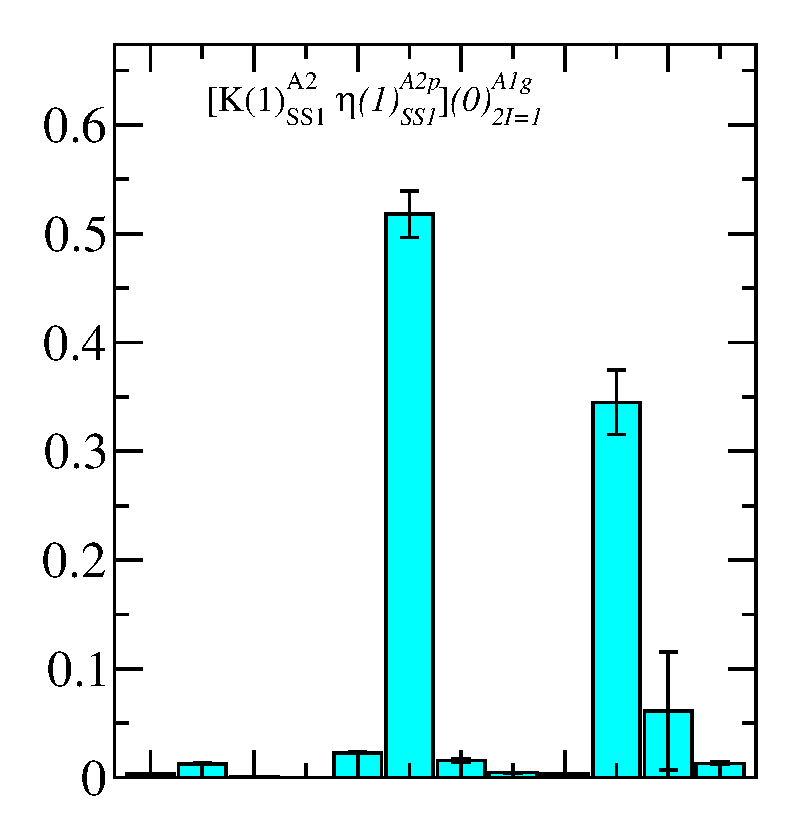
\includegraphics[width=0.28\textwidth]{figures/spectrum_a1g/with_tq/zfactors/zfactor_isodoublet_kaon_eta-A1g_1-P001-A2-SS_1-P00-1-A2p-SS_1.pdf}
  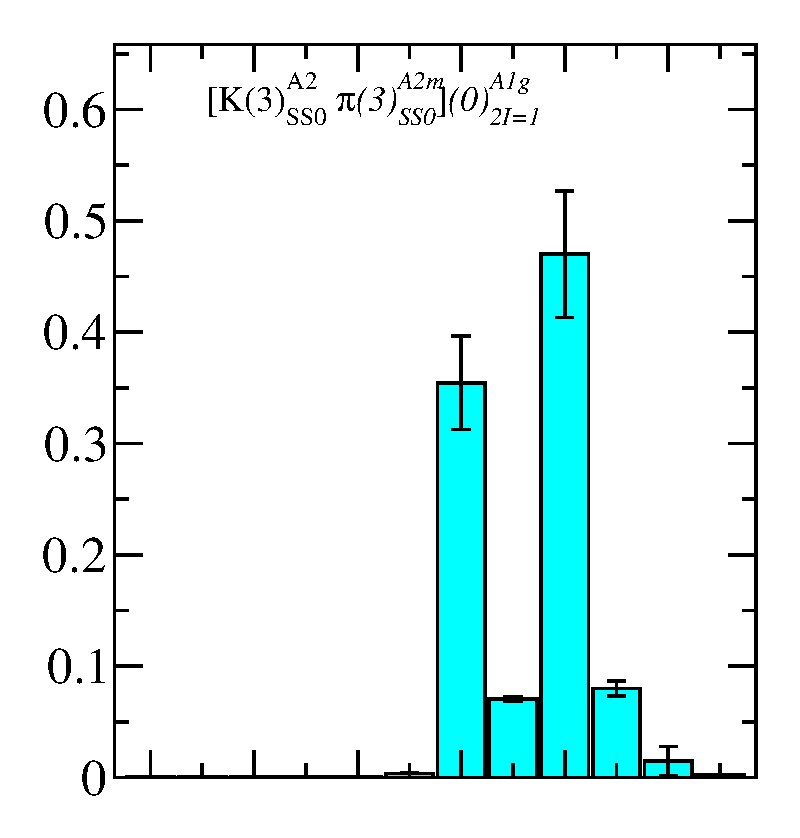
\includegraphics[width=0.28\textwidth]{figures/spectrum_a1g/with_tq/zfactors/zfactor_isodoublet_kaon_pion-A1g_1-P111-A2-SS_0-P-1-1-1-A2m-SS_0.pdf}\\
  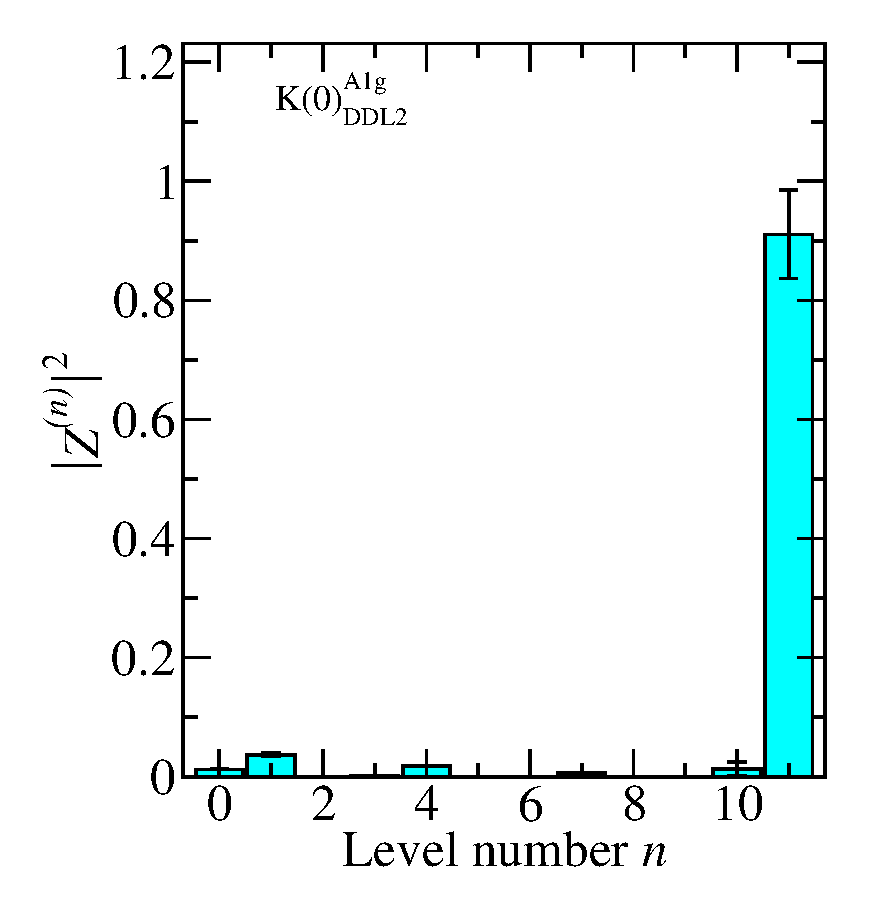
\includegraphics[width=0.304\textwidth]{figures/spectrum_a1g/with_tq/zfactors/zfactor_kaon-P000-A1g_1-DDL_2.pdf}
  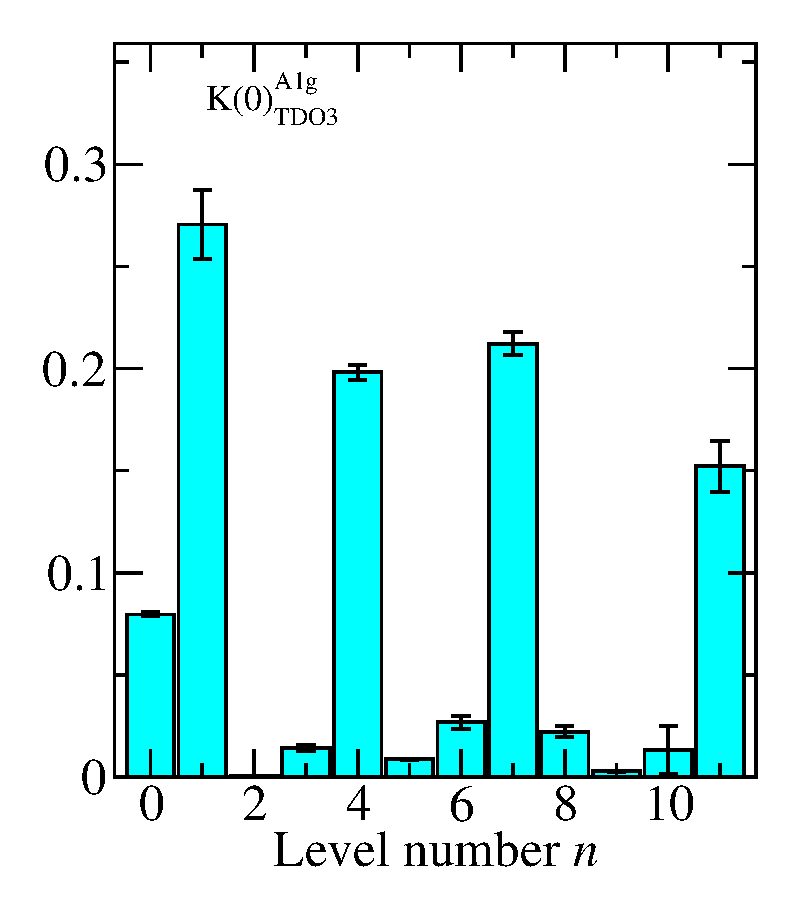
\includegraphics[width=0.28\textwidth]{figures/spectrum_a1g/with_tq/zfactors/zfactor_kaon-P000-A1g_1-TDO_3.pdf}
  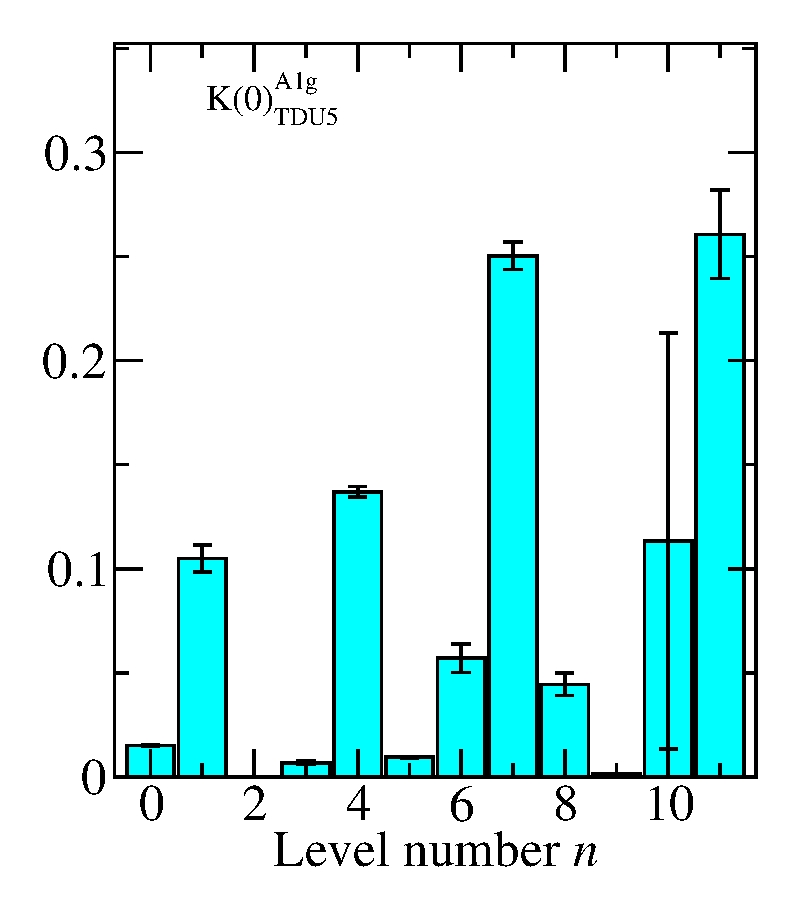
\includegraphics[width=0.28\textwidth]{figures/spectrum_a1g/with_tq/zfactors/zfactor_kaon-P000-A1g_1-TDU_5.pdf}
  \caption{Overlap factors for the operators used in the rotated $12\times 12$ correlator matrix in the $\kappa$ channel, using the operator basis given in Table~\ref{table:kappa_ops_no_tq}, but with the addition of one tetraquark operator.}
  \label{fig:kappa_with_tq_zfactors}
\end{figure}

\begin{table}
  \centering
  \begin{tabular}{c|c|c|c|c}
    $E / E_K$ & $a_t E$ & Fit model & $(t_{\mathrm{min}}, {t_\mathrm{max}})$ & $\chi^2 / \rm{d.o.f.}$\\
    \hline
    1.4685(64)&0.12259(53)&2{-}exp&$(7, 26)$&0.58\\
    1.914(31)&0.1598(26)&2{-}exp&$(8, 26)$&1.84\\
    1.951(69)&0.1629(57)&2{-}exp&$(4, 26)$&1.39\\
    2.139(62)&0.1786(52)&2{-}exp&$(7, 26)$&0.29\\
    2.397(18)&0.2001(14)&2{-}exp&$(4, 26)$&1.3\\
    2.567(33)&0.2143(27)&2{-}exp&$(5, 26)$&1.29\\
    2.79(15)&0.233(13)&1{-}exp&$(11, 26)$&1.37\\
    2.797(24)&0.2335(20)&2{-}exp&$(4, 26)$&1.71\\
    2.82(16)&0.235(13)&1{-}exp&$(11, 26)$&1.04\\
    3.291(95)&0.2748(80)&2{-}exp&$(3, 26)$&1.5
  \end{tabular}
  \caption{Fit details for the spectrum obtained in the $\kappa$ channel using the operator basis given in Table~\ref{table:kappa_ops_no_tq}, but with the addition of one tetraquark operator.}
  \label{table:kappa_with_tq_spectrum}
\end{table}

\begin{figure}
  \centering
  \hspace*{-0.5in}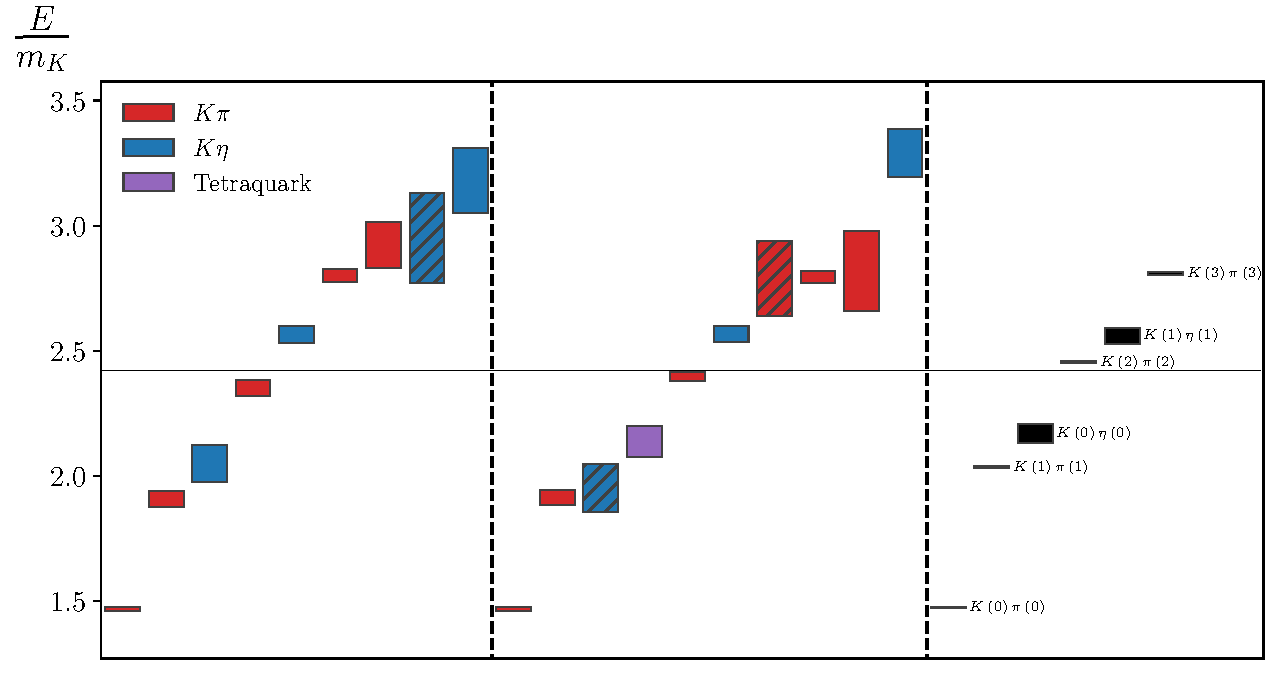
\includegraphics[width=\textwidth]{figures/spectrum_a1g/staircase.pdf}
  \caption[A comparison of spectrum determinations made in the $\kappa$ channel.]{On the left: an estimate of the spectrum obtained in the $\kappa$ channel using the operator basis given in Table~\ref{table:kappa_ops_no_tq}, which contains no tetraquark operators. In the middle: another estimate of the spectrum obtained in the $\kappa$ channel using the same basis but with the addition of one tetraquark operator. On the right: two-particle non-interacting energies calculated from the rest-frame masses of the constituent particles, up to the point at which we have confidently saturated the basis with two-particle operators. The horizontal dashed line indicates the four-particle $K\pi\pi\pi$ threshold. The color of a level indicates flavor content and is qualitatively determined by the overlap factors. If a level's overlap factor is dominant for operators of more than one flavor, then it is multi-colored. If the level also has significant (but not leading) overlap with a state created by an operator of a different flavor, then a hatched box is used to denote significant mixing.}
  \label{fig:kappa_spectrum}
\end{figure}

\begin{figure}
  \centering
  \hspace*{-0.5in}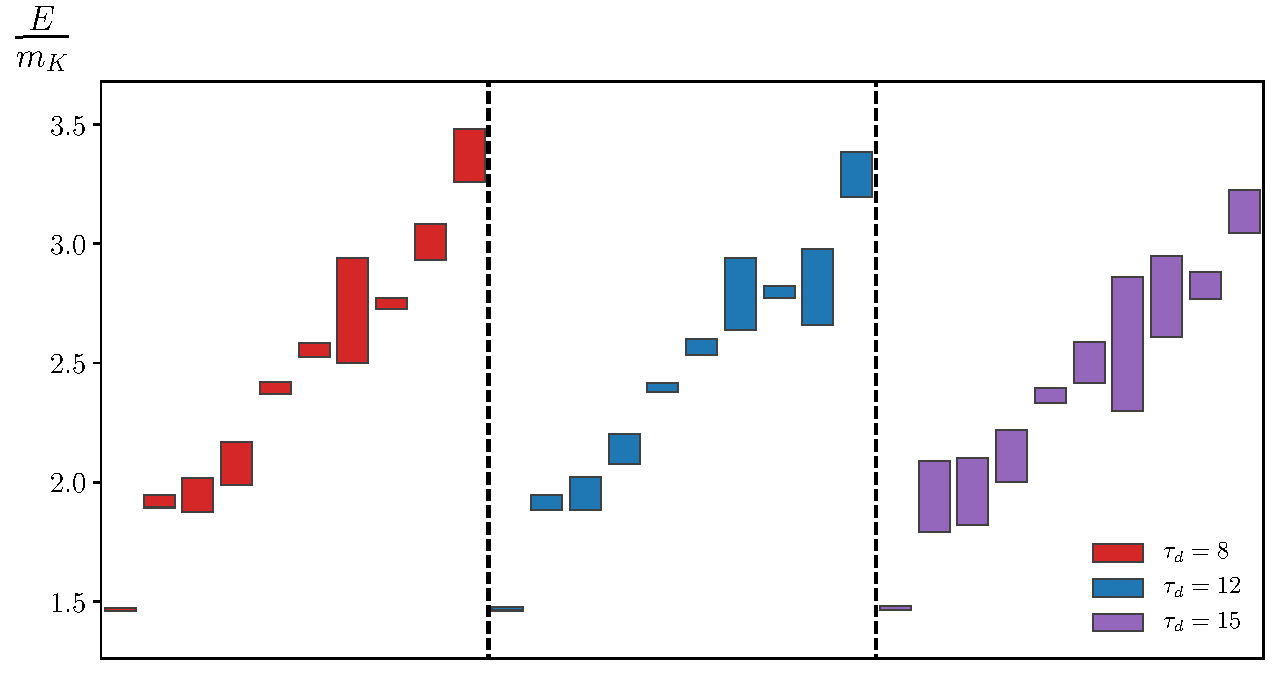
\includegraphics[width=\textwidth]{figures/spectrum_a1g/staircase_tau_d.pdf}
  \caption{Determinations of the spectrum obtained using three different diagonalization times, using the operator basis given in Table~\ref{table:kappa_ops_no_tq}, but with the addition of one tetraquark operator.}
  \label{fig:spectrum_td}
\end{figure}

\section{$a_0(980)$ Channel}\label{sec:a0}
\subsection{Operator Bases}
The quantum numbers associated with the $a_0(980)$ are $I^G(J^{PC}) = 1^-(0^{++})$ and $S = 0$, which means that on the lattice we work in the isotriplet, nonstrange, $A_{1g}^-$ symmetry sector (see Table~\ref{table:O_occurrence_nums}). Below a cutoff of approximately 1.5 times the mass of the nucleon, near where the $a_0(1450)$ appears, we expect to see two single-hadron states (the $a_0(980)$ and the $a_0(1450)$) and several multi-hadron states. The operator basis we use, not including any tetraquark operators, is shown in Table~\ref{table:a0_ops_no_tq}. We include two single-hadron operators (one triply-displaced and one singly-displaced) in hopes of capturing states corresponding to the $a_0(980)$ and the $a_0(1450)$. We attempted to include a single-site single-hadron operator, but doing so did not produce an operator set that was sufficiently linearly-independent and produced an effective mass that was indicative of a spurious state that was leaking to the ground state. This dramatically affected our ability to reliably extract the spectrum and caused it to be unstable under changes in the diagonalization time. Therefore, the single-site operator was discarded. As will be the case in Ch.~\ref{ch:sigmas}, we make use of so-called \emph{variationally improved} single-hadron operators. We obtain these operators by first diagonalizing in the subspace of single-hadron operators to form linear combinations with improved overlaps onto the single-hadron states of interest, in order to aid in level identification.

Our final class of tetraquark operators used in this channel were single-site $\overline u u \overline d u$, with both the symmetric and antisymmetric color structures included. The final tetraquark operator chosen was a $\overline u u \overline d u$, symmetric, single-site operator, which we denote as \verb+tquudu3p SS2+. Of the tetraquark operators that produced an additional level, we chose this one due to its high signal quality.
\begin{table}
  \centering
  \begin{tabular}{l|l}
    \textbf{Single-Hadron Operators} & \textbf{Two-Hadron Operators}\\
    \hline
    % $\pi^{\rm{TDO}3}_{A_{1g}^-}$ & $K(0)^{\rm{SS}0}_{A_{1u}}\; \overline K(0)^{\rm{SS}0}_{A_{1u}}$\\
    % $\pi^{\rm{SD}2}_{A_{1g}^-}$ & $K(1)^{\rm{SS}1}_{A_{2}}\; \overline K(1)^{\rm{SS}1}_{A_{2}}$ \\
    % & $K(2)^{\rm{SS}0}_{A_{2}}\; \overline K(2)^{\rm{SS}0}_{A_{2}}$ \\
    % & $K(2)^{\rm{SS}1}_{A_{2}}\; \overline K(2)^{\rm{SS}1}_{A_{2}}$ \\
    % & $\eta(0)^{\rm{SS}0}_{A_{1u}^+}\; \pi(0)^{\rm{SS}0}_{A_{1u}^-}$ \\
    % & $\phi(0)^{\rm{SS}0}_{A_{1u}^+}\; \pi(0)^{\rm{SS}0}_{A_{1u}^-}$ \\
    % & $\eta(1)^{\rm{SS}0}_{A_{2}^+}\; \pi(1)^{\rm{SS}0}_{A_{2}^-}$ \\
    % & $\phi(1)^{\rm{SS}1}_{A_{2}^+}\; \pi(1)^{\rm{SS}1}_{A_{2}^-}$ \\
    % & $\eta(2)^{\rm{SS}1}_{A_{2}^+}\; \pi(2)^{\rm{SS}1}_{A_{2}^-}$ \\
    % & $\phi(2)^{\rm{SS}0}_{A_{2}^+}\; \pi(2)^{\rm{SS}0}_{A_{2}^-}$ 
    $\pi_{A_{1g}^-}^{SD2}$ & $K(0)_{A_{1u}}^{SS0}\overline K(0)_{A_{1u}}^{SS0}$\\
$\pi_{A_{1g}^-}^{TDO3}$ & $K(1)_{A_2}^{SS1}\overline K(1)_{A_2}^{SS1}$\\
 & $K(2)_{A_2}^{SS0}\overline K(2)_{A_2}^{SS0}$\\
 & $K(2)_{A_2}^{SS1}\overline K(2)_{A_2}^{SS1}$\\
 & $\eta(0)_{A_{1u}^+}^{SS0}\pi(0)_{A_{1u}^-}^{SS0}$\\
 & $\eta(1)_{A_2^+}^{SS0}\pi(1)_{A_2^-}^{SS0}$\\
 & $\eta(2)_{A_2^+}^{SS1}\pi(2)_{A_2^-}^{SS1}$\\
 & $\phi(0)_{A_{1u}^+}^{SS0}\pi(0)_{A_{1u}^-}^{SS0}$\\
 & $\phi(1)_{A_2^+}^{SS1}\pi(1)_{A_2^-}^{SS1}$\\
 & $\phi(2)_{A_2^+}^{SS0}\pi(2)_{A_2^-}^{SS0}$

  \end{tabular}
  \caption[Operators used in the $a_0(980)$ channel, excluding tetraquark operators.]{Operators used in the $a_0(980)$ channel, excluding tetraquark operators. Particle names refer to \emph{flavor content} and should not be taken literally. $K$ refers to $u\overline s$, $\overline K$ refers to $s \overline u$, $\pi$ refers to $u\overline d$, $\eta$ refers to $u\overline u + d\overline d$, and $\phi$ refers to $s\overline s$ flavor structure. The number in parentheses following the particle name denotes the square of its total momentum in lattice units, the superscript denotes displacement type, and the subscript denotes octahedral irrep and $G$-parity.}
  \label{table:a0_ops_no_tq}
\end{table}
\subsection{Spectrum Determination}
In this channel, we used a normalization time, metric time, and diagonalization time of $\tau_N=3$, $\tau_0=4$, and $\tau_d=7$, respectively. We found these parameters yielded a sufficiently diagonal correlator matrix. Fits to the diagonalized correlator set for the operator basis containing no tetraquark operators are shown in Fig.~\ref{fig:a0_no_tq_grid}, and the operator overlap factors are shown in Fig.~\ref{fig:a0_no_tq_zfactors}. Fit details are given in Table~\ref{table:a0_no_tq_spectrum}. Fits to the same operator basis, but with the addition of the $\overline u u \overline d u$ tetraquark operator, are shown in Fig.~\ref{fig:a0_with_tq_grid}, and the operator overlap factors are shown in Fig.~\ref{fig:a0_with_tq_zfactors}. Fit details are given in Table~\ref{table:a0_with_tq_spectrum}.

As in the $\kappa$ channel, Fig.~\ref{fig:a0_spectrum} shows a comparison of our two estimates of the spectrum, one (left) obtained using only the operators in Table~\ref{table:a0_ops_no_tq}, the other (middle) obtained using the operator basis given in Table~\ref{table:a0_ops_no_tq} and the tetraquark operator. As in the $\kappa$ channel, we see an additional finite-volume state appear, however we see much more significant shifting of the other levels. We can attempt to explain this through level identification using the overlap factors in Figs.~\ref{fig:a0_no_tq_zfactors} and \ref{fig:a0_with_tq_zfactors}. In the spectrum obtained using the basis including the tetraquark operator, the ground state (level 0) most overlaps onto $\eta(0)\pi(0)$ and $\phi(0)\pi(0)$ operators, so we identify it as a physical $\pi(0)\eta(0)$ state. (Recall again that a physical $\eta$ meson is an admixture of the $\phi$ and $\eta$ flavor structures we use to define our operators.) Level 1 can clearly be identified as a $\overline K(0) K(0)$ state based on its overlap factor with the $\overline K(0) K(0)$ operator. Level 2 has the most significant overlap with the tetraquark operator, but also has significant mixing with the state created by the $\phi(0)\pi(0)$ operator. Levels 3, 4, 5, and 6 can be clearly identified as having $\phi\pi$, $\phi\pi$, $\overline K K$, and $\pi$ flavor structures, respectively, by inspecting the overlap factors. Importantly, our first variationally improved single-hadron operator \verb+ROT 0+ has a small but nonzero overlap with the tetraquark-dominated state, level 2, but has a leading overlap with level 6. (We will provisionally identify level 2 as the $a_0(980)$ and level 6 as the $a_0(1450)$.) When the tetraquark operator is not included, (see the left in Fig.~\ref{fig:a0_spectrum}), the \verb+ROT 0+ single-hadron operator does its best to produce both $a_0$ states, and we end up measuring a value for one mass between the two actual masses, such as explained in Ref.~\cite{Dudek:2012xn}. Similar shifting occurs in the $\phi\pi$-dominated levels 3 and 4, and in the $\overline K K$-dominated level 5. Once we add in the tetraquark operator, we have sufficiently saturated our basis to reliably resolve both $a_0$ states and accurately determine the spectrum. This significant result suggests that the $a_0(980)$ does indeed have significant tetraquark content. As with the $\kappa$ channel, a more detailed examination of the role of the tetraquark operator for the $a0(980)$ resonance will require the L\"uscher method with increased statistics and tetraquark operators of nonzero momenta. Additionally, our inability to reliably extract the spectrum without the addition of the tetraquark operator should cast doubt on any previous determinations of the spectrum in this channel made without the use of tetraquark operators.~\cite{Dudek:2016cru}


% most significantly overlaps onto level 4 (see Fig.~\ref{fig:a0_no_tq_zfactors}), but our second variationally improved operator does not have overlap onto either of these states. The tetraquark operator has \emph{significant} overlap onto the lower of the two $a_0$ states, while the single-hadron operator only has minimal overlap onto it. Therefore, without the tetraquark operator present, the single-hadron operator does its best to produce both $a_0$ states, and we end up measuring a value for one mass between the two actual masses, such as explained in Ref.~\cite{Dudek:2012xn}. Once we add in the tetraquark operator, we have sufficiently saturated our basis to reliably resolve both $a_0$ states. This is highly suggestive that the $a_0(980)$ does indeed have significant tetraquark content. As with the $\kappa$ channel, firm evidence for tetraquark content of the $a_0(980)$ resonance in infinite-volume will have to wait for future scattering studies.

\begin{figure}
  \raisebox{0cm}{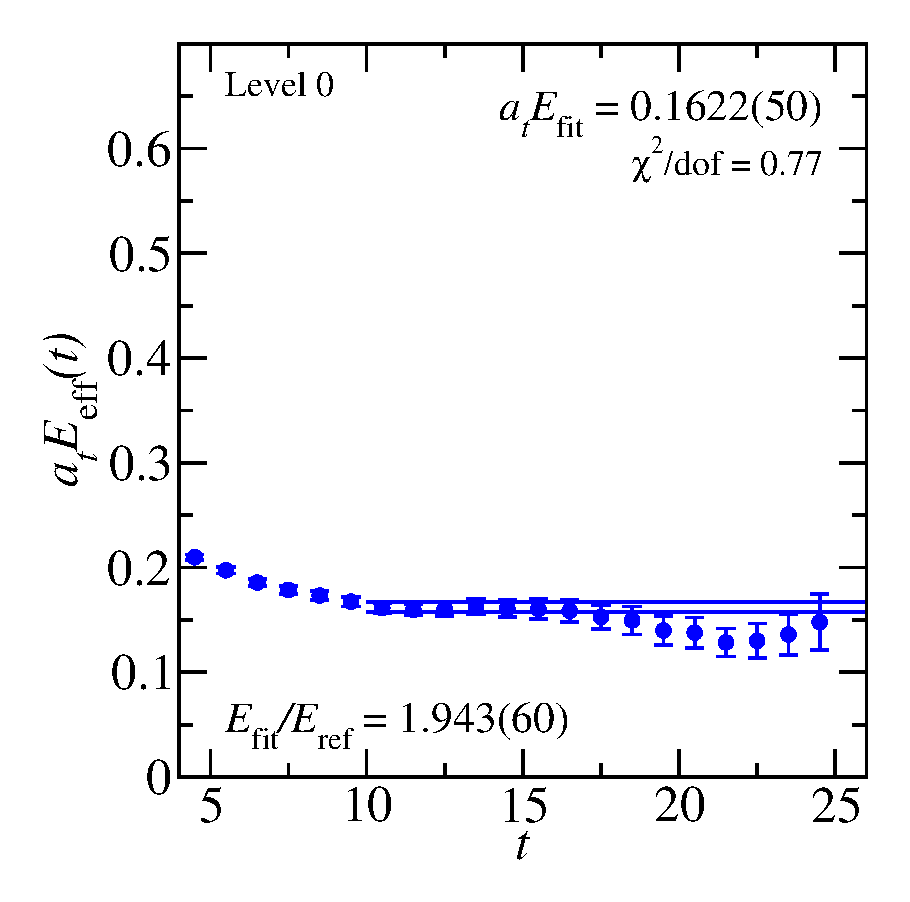
\includegraphics[width=0.329\textwidth]{figures/spectrum_a1gm/no_tq/fits/fit_0.pdf}}
  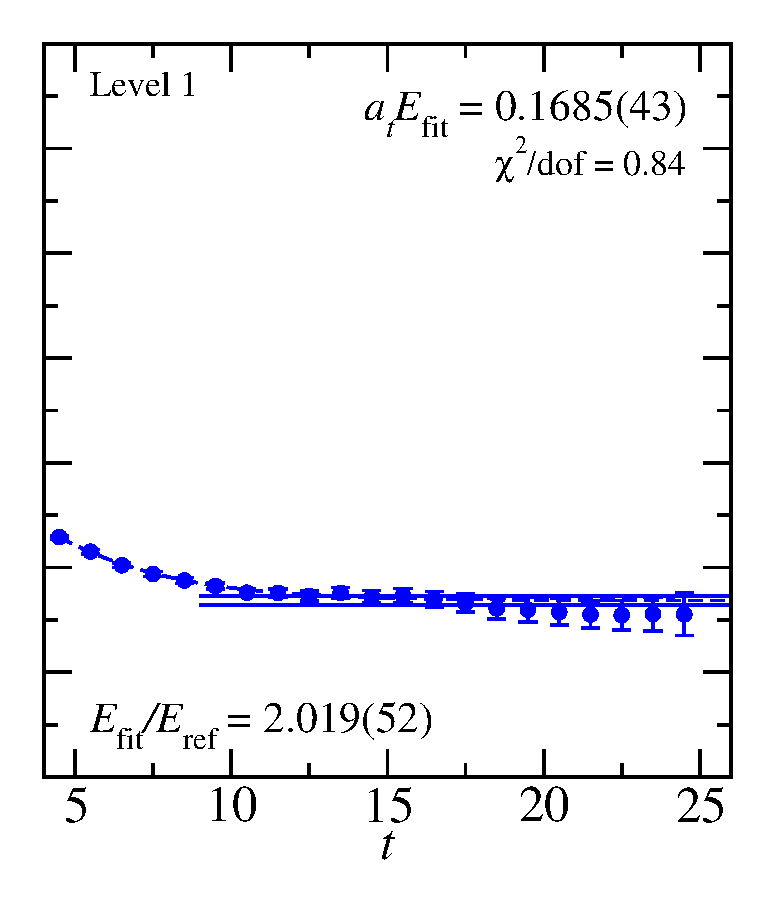
\includegraphics[width=0.28\textwidth]{figures/spectrum_a1gm/no_tq/fits/fit_1.pdf}
  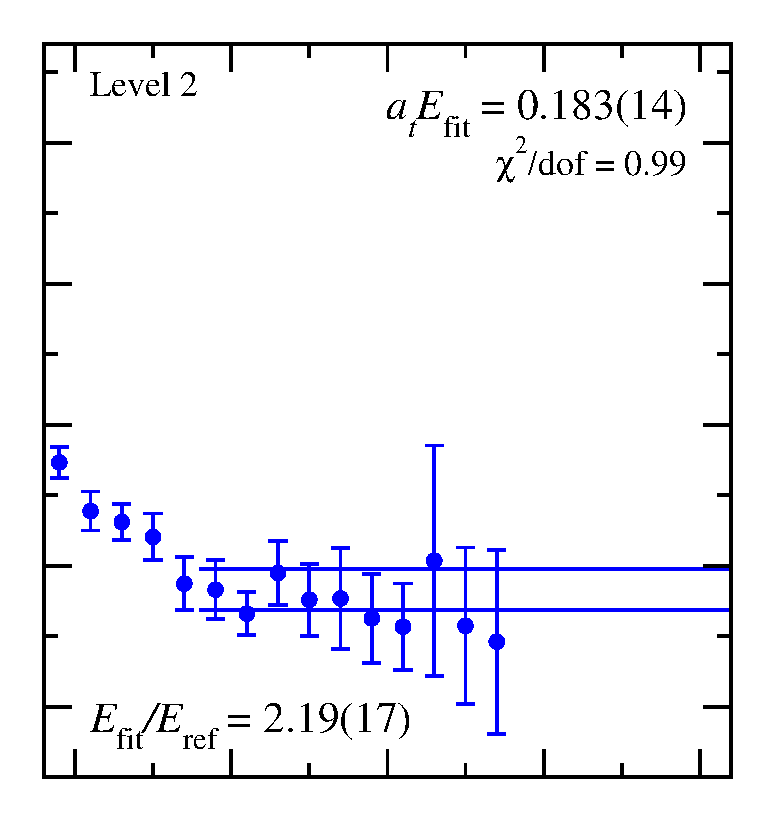
\includegraphics[width=0.28\textwidth]{figures/spectrum_a1gm/no_tq/fits/fit_2.pdf}\\
  \raisebox{-0.0in}{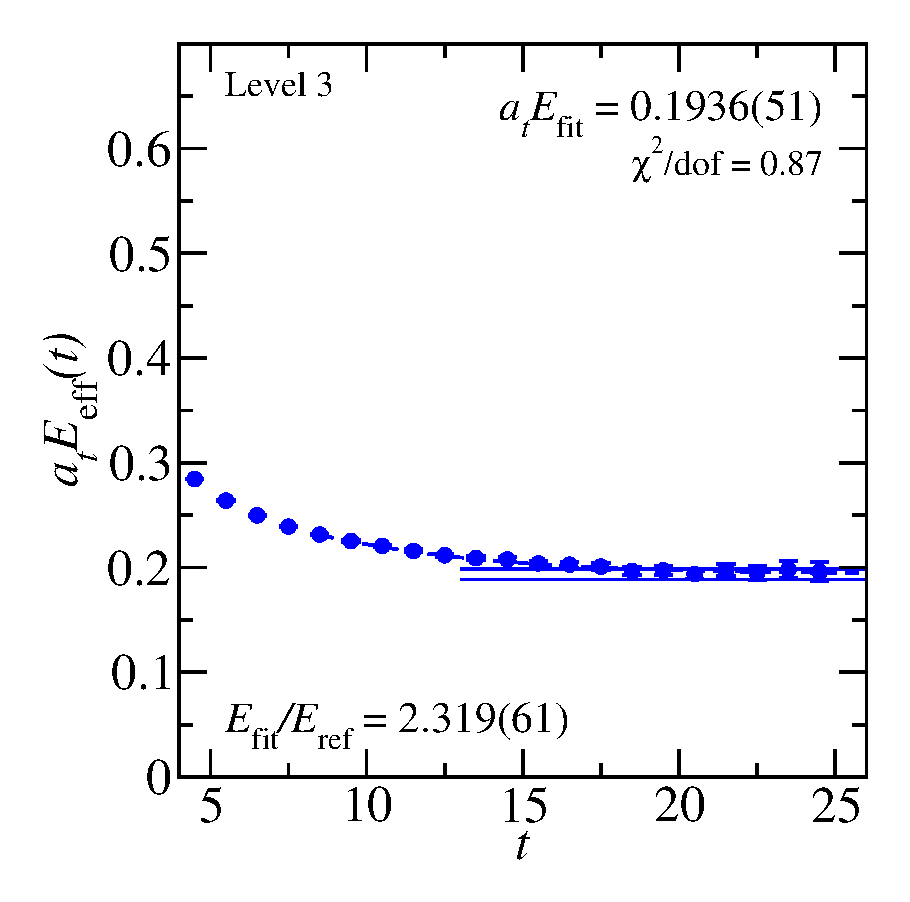
\includegraphics[width=0.329\textwidth]{figures/spectrum_a1gm/no_tq/fits/fit_3.pdf}}
  \includegraphics[width=0.28\textwidth]{figures/spectrum_a1gm/no_tq/fits/fit_5.pdf}
  \includegraphics[width=0.28\textwidth]{figures/spectrum_a1gm/no_tq/fits/fit_4.pdf}\\
  \raisebox{-0.00in}{\includegraphics[width=0.329\textwidth]{figures/spectrum_a1gm/no_tq/fits/fit_6.pdf}}
  \includegraphics[width=0.28\textwidth]{figures/spectrum_a1gm/no_tq/fits/fit_7.pdf}
  \includegraphics[width=0.28\textwidth]{figures/spectrum_a1gm/no_tq/fits/fit_8.pdf}\\
  \caption[Effective energies for the rotated $12\times 12$ correlator matrix in the $a_0(980)$ channel, using the operator basis given in Table~\ref{table:a0_ops_no_tq}, which contains no tetraquark operators.]{Effective energies for the rotated $12\times 12$ correlator matrix in the $a_0(980)$ channel, using the operator basis given in Table~\ref{table:a0_ops_no_tq}, which contains no tetraquark operators. Effective energy curves calculated from correlator fits are overlaid, and fit results are shown. For all effective mass plots in this work, a time step of $\Delta t = 3$ is used for the discretized derivative.}
  \label{fig:a0_no_tq_grid}
\end{figure}

\begin{figure}
  \includegraphics[width=0.304\textwidth]{figures/spectrum_a1gm/no_tq/zfactors/zfactor_isotriplet-S0-P000-A1gm_1-ROT-0.pdf}
  \includegraphics[width=0.28\textwidth]{figures/spectrum_a1gm/no_tq/zfactors/zfactor_isotriplet-S0-P000-A1gm_1-ROT-1.pdf}
  \includegraphics[width=0.28\textwidth]{figures/spectrum_a1gm/no_tq/zfactors/zfactor_isotriplet_phi_pion-A1gm_1-P000-A1up-SS_0-P000-A1um-SS_0.pdf}\\
  \includegraphics[width=0.304\textwidth]{figures/spectrum_a1gm/no_tq/zfactors/zfactor_isotriplet_eta_pion-A1gm_1-P000-A1up-SS_0-P000-A1um-SS_0.pdf}
  \includegraphics[width=0.28\textwidth]{figures/spectrum_a1gm/no_tq/zfactors/zfactor_isotriplet_kaon_kbar-A1gm_1-P000-A1u-SS_0-P000-A1u-SS_0.pdf}
  \includegraphics[width=0.28\textwidth]{figures/spectrum_a1gm/no_tq/zfactors/zfactor_isotriplet_phi_pion-A1gm_1-P001-A2p-SS_1-P00-1-A2m-SS_1.pdf}\\
  \includegraphics[width=0.304\textwidth]{figures/spectrum_a1gm/no_tq/zfactors/zfactor_isotriplet_kaon_kbar-A1gm_1-P001-A2-SS_1-P00-1-A2-SS_1.pdf}
  \includegraphics[width=0.28\textwidth]{figures/spectrum_a1gm/no_tq/zfactors/zfactor_isotriplet_phi_pion-A1gm_1-P011-A2p-SS_0-P0-1-1-A2m-SS_0.pdf}
  \includegraphics[width=0.28\textwidth]{figures/spectrum_a1gm/no_tq/zfactors/zfactor_isotriplet_eta_pion-A1gm_1-P001-A2p-SS_0-P00-1-A2m-SS_0.pdf}\\
  \includegraphics[width=0.304\textwidth]{figures/spectrum_a1gm/no_tq/zfactors/zfactor_isotriplet_eta_pion-A1gm_1-P011-A2p-SS_1-P0-1-1-A2m-SS_1.pdf}
  \includegraphics[width=0.28\textwidth]{figures/spectrum_a1gm/no_tq/zfactors/zfactor_isotriplet_kaon_kbar-A1gm_1-P011-A2-SS_0-P0-1-1-A2-SS_0.pdf}
  \includegraphics[width=0.28\textwidth]{figures/spectrum_a1gm/no_tq/zfactors/zfactor_isotriplet_kaon_kbar-A1gm_1-P011-A2-SS_1-P0-1-1-A2-SS_1.pdf}
  \cprotect\caption[Overlap factors for the operators used in the rotated $12\times 12$ correlator matrix in the $a_0(980)$ channel, using the operators in Table~\ref{table:a0_ops_no_tq}, which contains no tetraquark operators.]{Overlap factors for the operators used in the rotated $12\times 12$ correlator matrix in the $a_0(980)$ channel, using the operators in Table~\ref{table:a0_ops_no_tq}, which contains no tetraquark operators. Operators labeled by \verb+ROT N+ denote our variationally improved single-hadron operators.}
  \label{fig:a0_no_tq_zfactors}
\end{figure}

\begin{table}
  \centering
  \begin{tabular}{c|c|c|c|c}
    $E / E_K$ & $a_t E$ & Fit model & $(t_{\mathrm{min}}, {t_\mathrm{max}})$ & $\chi^2 / \rm{d.o.f.}$\\
    \hline
    1.475(74)&0.1231(62)&2{-}exp&$(3, 26)$&1.13\\
    2.034(25)&0.1698(21)&2{-}exp&$(5, 26)$&1.3\\
    2.19(17)&0.183(14)&1{-}exp&$(9, 26)$&0.99\\
    2.224(35)&0.1857(29)&2{-}exp&$(6, 26)$&1.08\\
    2.30(15)&0.192(13)&2{-}exp&$(6, 26)$&0.81\\
    2.452(33)&0.2047(27)&2{-}exp&$(6, 26)$&0.45\\
    2.828(45)&0.2361(37)&2{-}exp&$(6, 26)$&0.71\\
    2.971(32)&0.2480(26)&2{-}exp&$(4, 26)$&1.66\\
    5.00(39)&0.417(33)&1{-}exp&$(8, 18)$&1.23
  \end{tabular}
  \caption{Fit details for the determination of the spectrum obtained in the $a_0(980)$ channel, using the operator basis given in Table~\ref{table:a0_ops_no_tq}, which contains no tetraquark operators.}
  \label{table:a0_no_tq_spectrum}
\end{table}

\begin{figure}
  \includegraphics[width=0.329\textwidth]{figures/spectrum_a1gm/with_tq/fits/fit_0.pdf}
  \includegraphics[width=0.28\textwidth]{figures/spectrum_a1gm/with_tq/fits/fit_2.pdf}
  \includegraphics[width=0.28\textwidth]{figures/spectrum_a1gm/with_tq/fits/fit_1.pdf}\\
  \includegraphics[width=0.329\textwidth]{figures/spectrum_a1gm/with_tq/fits/fit_3.pdf}
  \includegraphics[width=0.28\textwidth]{figures/spectrum_a1gm/with_tq/fits/fit_4.pdf}
  \includegraphics[width=0.28\textwidth]{figures/spectrum_a1gm/with_tq/fits/fit_5.pdf}\\
  \raisebox{0.48cm}{\includegraphics[width=0.329\textwidth]{figures/spectrum_a1gm/with_tq/fits/fit_6.pdf}}
  \includegraphics[width=0.28\textwidth]{figures/spectrum_a1gm/with_tq/fits/fit_7.pdf}
  \includegraphics[width=0.28\textwidth]{figures/spectrum_a1gm/with_tq/fits/fit_8.pdf}\\[-0.4cm]
  \includegraphics[width=0.329\textwidth]{figures/spectrum_a1gm/with_tq/fits/fit_9.pdf}
  \caption[Effective energies for the rotated $13\times 13$ correlator matrix in the $a_0(980)$ channel, using the operator basis given in Table~\ref{table:a0_ops_no_tq}, but with the addition of one tetraquark operator.]{Effective energies for the rotated $13\times 13$ correlator matrix in the $a_0(980)$ channel, using the operator basis given in Table~\ref{table:a0_ops_no_tq}, but with the addition of one tetraquark operator. Effective energy curves calculated from correlator fits are overlaid, and fit results are shown.}
  \label{fig:a0_with_tq_grid}
\end{figure}

\begin{figure}
  \includegraphics[width=0.24\textwidth]{figures/spectrum_a1gm/with_tq/zfactors/zfactor_isotriplet-S0-P000-A1gm_1-ROT-0.pdf}
  \includegraphics[width=0.22\textwidth]{figures/spectrum_a1gm/with_tq/zfactors/zfactor_isotriplet-S0-P000-A1gm_1-ROT-1.pdf}
  \includegraphics[width=0.22\textwidth]{figures/spectrum_a1gm/with_tq/zfactors/zfactor_tquudu3p-P000-A1gm_1-SS_2.pdf}
  \includegraphics[width=0.22\textwidth]{figures/spectrum_a1gm/with_tq/zfactors/zfactor_isotriplet_phi_pion-A1gm_1-P000-A1up-SS_0-P000-A1um-SS_0.pdf}\\
  \includegraphics[width=0.24\textwidth]{figures/spectrum_a1gm/with_tq/zfactors/zfactor_isotriplet_eta_pion-A1gm_1-P000-A1up-SS_0-P000-A1um-SS_0.pdf}
  \includegraphics[width=0.22\textwidth]{figures/spectrum_a1gm/with_tq/zfactors/zfactor_isotriplet_kaon_kbar-A1gm_1-P000-A1u-SS_0-P000-A1u-SS_0.pdf}
  \includegraphics[width=0.22\textwidth]{figures/spectrum_a1gm/with_tq/zfactors/zfactor_isotriplet_phi_pion-A1gm_1-P001-A2p-SS_1-P00-1-A2m-SS_1.pdf}
  \includegraphics[width=0.22\textwidth]{figures/spectrum_a1gm/with_tq/zfactors/zfactor_isotriplet_kaon_kbar-A1gm_1-P001-A2-SS_1-P00-1-A2-SS_1.pdf}\\
  \raisebox{0.12in}{\includegraphics[width=0.24\textwidth]{figures/spectrum_a1gm/with_tq/zfactors/zfactor_isotriplet_phi_pion-A1gm_1-P011-A2p-SS_0-P0-1-1-A2m-SS_0.pdf}}
  \includegraphics[width=0.22\textwidth]{figures/spectrum_a1gm/with_tq/zfactors/zfactor_isotriplet_eta_pion-A1gm_1-P001-A2p-SS_0-P00-1-A2m-SS_0.pdf}
  \includegraphics[width=0.22\textwidth]{figures/spectrum_a1gm/with_tq/zfactors/zfactor_isotriplet_eta_pion-A1gm_1-P011-A2p-SS_1-P0-1-1-A2m-SS_1.pdf}
  \includegraphics[width=0.22\textwidth]{figures/spectrum_a1gm/with_tq/zfactors/zfactor_isotriplet_kaon_kbar-A1gm_1-P011-A2-SS_0-P0-1-1-A2-SS_0.pdf}\\[-0.2cm]
  \includegraphics[width=0.24\textwidth]{figures/spectrum_a1gm/with_tq/zfactors/zfactor_isotriplet_kaon_kbar-A1gm_1-P011-A2-SS_1-P0-1-1-A2-SS_1.pdf}
  \cprotect\caption[Overlap factors for the operators used in the rotated $13\times 13$ correlator matrix in the $a_0(980)$ channel, using the operator basis given in Table~\ref{table:a0_ops_no_tq}, but with the addition of one tetraquark operator.]{Overlap factors for the operators used in the rotated $13\times 13$ correlator matrix in the $a_0(980)$ channel, using the operator basis given in Table~\ref{table:a0_ops_no_tq}, but with the addition of one tetraquark operator. Operators labeled by \verb+ROT N+ denote our variationally improved single-hadron operators.}
  \label{fig:a0_with_tq_zfactors}
\end{figure}

\begin{table}
  \centering
  \begin{tabular}{c|c|c|c|c}
    $E / E_K$ & $a_t E$ & Fit model & $(t_{\mathrm{min}}, {t_\mathrm{max}})$ & $\chi^2 / \rm{d.o.f.}$\\
    \hline
    1.410(79)&0.1177(66)&2{-}exp&$(3, 26)$&1.12\\
    2.014(29)&0.1681(24)&2{-}exp&$(6, 26)$&1.99\\
    2.03(11)&0.1692(92)&2{-}exp&$(3, 26)$&1.03\\
    2.41(13)&0.201(11)&1{-}exp&$(9, 26)$&0.82\\
    2.537(42)&0.2118(35)&2{-}exp&$(3, 26)$&1.18\\
    2.586(26)&0.2159(21)&2{-}exp&$(4, 26)$&0.67\\
    2.84(12)&0.237(10)&2{-}exp&$(3, 24)$&0.99\\
    2.947(40)&0.2461(33)&2{-}exp&$(4, 26)$&0.9\\
    2.964(35)&0.2475(29)&2{-}exp&$(4, 26)$&1.64\\
    5.01(39)&0.418(33)&1{-}exp&$(8, 18)$&1.25
  \end{tabular}
  \caption{Fit details for the spectrum obtained in the $a_0(980)$ channel using the operator basis given in Table~\ref{table:a0_ops_no_tq}, but with the addition of one tetraquark operator.}
  \label{table:a0_with_tq_spectrum}
\end{table}

\begin{figure}
  \centering
  \hspace*{-0.5in}\includegraphics[width=\textwidth]{figures/spectrum_a1gm/staircase.pdf}
  \caption[A comparison of spectrum determinations made in the $a_0(980)$ channel.]{On the left: an estimate of the spectrum obtained in the $a_0(980)$ channel using the operator basis given in Table~\ref{table:a0_ops_no_tq}, which contains no tetraquark operators. In the middle: another estimate of the spectrum obtained in the $a_0(980)$ channel using the same basis but with the addition of one tetraquark operator. On the right: two-particle non-interacting energies calculated from the rest-frame masses of the constituent particles, up to the point at which we have confidently saturated the basis with two-particle operators. The horizontal dash line indicates the four-particle $\pi\pi\pi\eta$ threshold. The color of a level indicates flavor content and is qualitatively determined by the overlap factors. If a level's overlap factor is dominant for operators of more than one flavor, then it is multi-colored. If the level also has significant (but not leading) overlap with a state created by an operator of a different flavor, then a hatched box is used to denote significant mixing.}
  \label{fig:a0_spectrum}
\end{figure}